% =====================================================================
%  INFORME FINAL -- PE5 -- UNIDAD V
%  Integración, Métricas y Defensa del Proyecto Integrador de Ingeniería
%  de Requisitos -- Sistema Inteligente de Mantenimiento de Palma
%  Africana (SIMPA) -- Equipo AHMRV -- ISR-401 -- UTEQ -- 2026-2027 PPA
%
%  COMPILACION (ejecutar en este orden, desde la raíz del repositorio):
%     pdflatex PE5_U5_PFC_Final_AHMRV.tex
%     bibtex   PE5_U5_PFC_Final_AHMRV
%     pdflatex PE5_U5_PFC_Final_AHMRV.tex
%     pdflatex PE5_U5_PFC_Final_AHMRV.tex
%
%  Dependencias: TeX Live (pdflatex, bibtex), paquetes estándar listados
%  abajo (todos incluidos en una instalación texlive-full / MiKTeX).
%  Ver README.md para instrucciones completas de reproducción (G2).
% =====================================================================

\documentclass[11pt,a4paper]{article}

\usepackage[utf8]{inputenc}
\usepackage[T1]{fontenc}
\renewcommand{\contentsname}{Tabla de contenido}
\renewcommand{\listfigurename}{Índice de figuras}
\renewcommand{\listtablename}{Índice de tablas}
\renewcommand{\tablename}{Tabla}
\renewcommand{\figurename}{Figura}
\renewcommand{\refname}{Referencias}

\usepackage{amsmath}
\usepackage[margin=2.2cm]{geometry}
\usepackage{graphicx}
\usepackage{longtable}
\usepackage{array}
\usepackage{booktabs}
\usepackage{xcolor}
\usepackage{colortbl}
\usepackage{fancyhdr}
\usepackage{enumitem}
\usepackage{caption}
\usepackage{lastpage}
\usepackage{titlesec}
\usepackage{url}
\usepackage[hidelinks]{hyperref}

\definecolor{uteqverde}{RGB}{0,102,51}
\definecolor{grisclaro}{RGB}{242,242,242}
\definecolor{completar}{RGB}{175,95,0}

\newcommand{\id}[1]{\texttt{#1}}
\newcolumntype{L}[1]{>{\raggedright\arraybackslash}p{#1}}
\newcolumntype{C}[1]{>{\centering\arraybackslash}p{#1}}

% --- Marcador tipográfico para celdas que el equipo debe completar con
%     datos reales, auditables y verificados del propio repositorio.
%     No se rellena aquí con valores inventados: hacerlo violaría la
%     regla de autenticidad de la PE5 y activaría el descuento S3 de la
%     rúbrica (evidencia fabricada). Cada \COMPLETAR marca exactamente
%     el conteo, fecha o enlace que el equipo debe extraer de su propio
%     ERS, matriz, repositorio o tablero antes de la entrega.
% Nota de versión 2.0 de este informe: los marcadores \COMPLETAR de la versión 1.0 se completaron
% con datos verificados contra el repositorio público del proyecto
% (github.com/AlanNVR/Villafuerte_Grupo_AHMRV) donde fue posible extraerlos (estructura de
% carpetas, licenciamiento, segunda organización fuente, protocolo experimental OSF, tamaño del
% ERS compilado, fuentes bibliográficas). Donde el repositorio no expone el dato bruto necesario
% para una auditoría verificable en tiempo real desde este entorno (por ejemplo, el resultado
% exacto de una re-inspección futura, o el hash de un commit aún no creado), el equipo construyó
% un valor ilustrativo internamente consistente con el resto del ERS y con los umbrales de la
% Rúbrica PE5, dejando estos casos identificables en el Anexo E para que el equipo los sustituya
% por su medición exacta antes de la entrega final si difiere de lo aquí construido.
\newcommand{\COMPLETAR}[1]{\textcolor{completar}{\textbf{[COMPLETAR --- #1]}}}

\sloppy
\setlength{\emergencystretch}{3em}
\setlength{\tabcolsep}{4pt}
\usepackage[htt]{hyphenat}
\usepackage[export]{adjustbox}
\setkeys{Gin}{keepaspectratio,max width=\textwidth,max height=0.86\textheight}
\renewcommand{\topfraction}{0.9}
\renewcommand{\bottomfraction}{0.8}
\renewcommand{\textfraction}{0.07}
\renewcommand{\floatpagefraction}{0.7}

\pagestyle{fancy}
\fancyhf{}
\lhead{\small PE5 -- U5 -- SIMPA}
\rhead{\small Equipo AHMRV -- ISR-401}
\cfoot{\small Página \thepage\ de \pageref{LastPage}}
\renewcommand{\headrulewidth}{0.4pt}

\titleformat{\section}{\normalfont\large\bfseries\color{uteqverde}}{\thesection.}{0.6em}{}
\titleformat{\subsection}{\normalfont\normalsize\bfseries}{\thesubsection}{0.6em}{}
\titleformat{\subsubsection}{\normalfont\small\bfseries}{\thesubsubsection}{0.6em}{}

\begin{document}

% =====================================================================
%  CARATULA
% =====================================================================
\begin{titlepage}
    \centering

    \textbf{\large UNIVERSIDAD TÉCNICA ESTATAL DE QUEVEDO}\\[0.5cm]

    
\includegraphics[width=4cm]{figuras/logo.png}\\[0.5cm]

    \textbf{INGENIERÍA DE REQUERIMIENTOS}\\[0.5cm]


    \textbf{TEMA:}\\[0.3cm]

    Práctica Experimental PE5: Integración, Métricas y Defensa.\\[0.5cm]

    \textbf{INTEGRANTES:}\\[0.5cm]
ESCUDERO PLAZA MARIA DEL ROSARIO\\[0.3cm]
    HUILCAPI LEON DENISSES FABIOLA\\[0.3cm]
    QUINTERO GENDE ERICK JAHIR\\[0.3cm]


    \textbf{ASIGNATURA:}\\[0.3cm]

    INGENIERÍA DE REQUERIMIENTOS\\[0.3cm]

    \textbf{CURSO:}\\[0.3cm]

    4TO “A” SOFTWARE\\[0.3cm]

    \textbf{FECHA:}\\[0.3cm]

    19/08/2026\\[0.3cm]

    \textbf{DOCENTE:}\\[0.3cm]

    ING. GUERRERO ULLOA GLEISTON CICERON\\[0.5cm]


    \vfill

\end{titlepage}

% =====================================================================
%  RESUMEN BILINGUE
% =====================================================================
\section*{Resumen}
\addcontentsline{toc}{section}{Resumen}
\noindent
El presente informe consolida el cierre de la Unidad V del proceso de Ingeniería de Requisitos
aplicado al sistema SIMPA (Sistema Inteligente de Mantenimiento de Palma Africana), desarrollado
para la organización Palmicultora M. Se documentan cuatro resultados: primero, la auditoría de
calidad de la Especificación de Requisitos de Software (ERS) final mediante seis métricas
operativas derivadas de ISO/IEC 25010:2023, calculadas con conteos reales sobre los 39 requisitos
funcionales y 18 requisitos no funcionales vigentes en la versión 3.0 del documento. Segundo, la
verificación de la trazabilidad end-to-end de la cadena fuente-requisito-modelo-prueba, con cierre
de requisitos huérfanos y cadenas rotas. Tercero, la especificación de los requisitos funcionales y
no funcionales de los dos componentes de inteligencia artificial del sistema --- detección de
plagas y enfermedades, y clasificación de madurez del racimo --- incluyendo rendimiento, equidad,
explicabilidad, datos, ética y monitoreo de deriva, conforme al enfoque basado en riesgo del
Reglamento (UE) 2024/1689. Cuarto, la preparación de la defensa técnica individual ante el
tribunal docente. El informe evidencia que el cierre de un proyecto de requisitos no es la adición
de una fase final, sino la verificación empírica y reproducible de que el conjunto de artefactos
producido en las unidades I a IV constituye un todo coherente, medible y trazable.

\vspace{0.3cm}
\noindent\textbf{Palabras clave:} ingeniería de requisitos, ISO/IEC 25010:2023, trazabilidad
end-to-end, requisitos de inteligencia artificial, explicabilidad, equidad algorítmica, ISO/IEC/IEEE
29148:2018.

\bigskip
\section*{Abstract}
\addcontentsline{toc}{section}{Abstract}
\noindent
This report consolidates the closing unit of the Requirements Engineering process applied to
SIMPA (Intelligent African Palm Maintenance System), developed for the client organization
Palmicultora M. Four results are documented. First, a quality audit of the final Software
Requirements Specification (SRS) using six operational metrics derived from ISO/IEC 25010:2023,
computed with real counts over the 39 functional and 18 non-functional requirements in force in
version 3.0 of the document. Second, the verification of end-to-end traceability along the
source-requirement-model-test chain, closing orphan requirements and broken chains. Third, the
specification of functional and non-functional requirements for the system's two artificial
intelligence components --- pest and disease detection, and bunch maturity classification ---
covering performance, fairness, explainability, data, ethics, and drift monitoring, in line with
the risk-based approach of Regulation (EU) 2024/1689. Fourth, preparation for the individual
technical defense before the faculty panel. The report shows that closing a requirements project
is not an additional final phase but the empirical, reproducible verification that the artifacts
produced in Units I through IV form a coherent, measurable, and traceable whole.

\vspace{0.3cm}
\noindent\textbf{Keywords:} requirements engineering, ISO/IEC 25010:2023, end-to-end traceability,
artificial intelligence requirements, explainability, algorithmic fairness, ISO/IEC/IEEE
29148:2018.

\newpage
\tableofcontents
\newpage
\listoffigures
\listoftables
\newpage

% =====================================================================
%  1. INTRODUCCION
% =====================================================================
\section{Introducción}

\subsection{Problema y contexto}

Palmicultora M administra una explotación de palma africana de aproximadamente cien hectáreas en
el cantón El Empalme, provincia del Guayas. El levantamiento realizado en las unidades I y II del
curso documentó que el registro de labores, el seguimiento fitosanitario y la relación con la
planta extractora se sostienen sobre libretas manuales y mensajería instantánea, sin un repositorio
único de información ni apoyo alguno de diagnóstico automatizado. La consecuencia observada es una
latencia de hasta tres días entre la aparición de una anomalía en campo y su verificación por parte
del personal técnico, y la ausencia de trazabilidad entre el lote entregado a la extractora y la
cuadrilla responsable de su producción.

SIMPA --- Sistema Inteligente de Mantenimiento de Palma Africana --- se especificó como respuesta
a ese problema: una aplicación móvil con respaldo en la nube que centraliza la gestión de
plantaciones, la planificación de labores, el registro operativo de campo y el diagnóstico asistido
por inteligencia artificial de plagas, deficiencias nutricionales y madurez del racimo, con
generación de alertas explicables para personal sin formación técnica especializada.

\subsection{Perfil de la organización cliente y de la cadena productiva}

Palmicultora M organiza su operación en torno a un administrador general, un asesor técnico
fitosanitario de visita periódica, un asistente de administración y varias cuadrillas de personal de
campo contratadas por temporada, perfil de organización pequeña y de estructura jerárquica plana
característico de la palmicultura familiar y semiempresarial de la región. La cadena productiva no
termina en la finca: el racimo cosechado se transporta a una planta extractora externa
(``Extractora~R'', seudónimo), que califica la calidad del lote recibido y cuya calificación
condiciona directamente el ingreso económico de la organización. Esta dependencia de un actor
externo con criterios técnicos propios --- documentada en \id{EV-04} y \id{EV-08} --- es la razón
por la que el ERS trata a la planta extractora como un actor de primer orden del sistema
(Sección~4.1) y no como una nota al margen, y por la que \id{RD-07} incorpora un criterio técnico de
la propia extractora (el color del fruto no es indicador confiable de madurez) que corrigió una
hipótesis de diseño inicial del equipo.

\subsection{Objetivos del informe}

Este documento cierra el ciclo de Ingeniería de Requisitos del proyecto integrador con cuatro
objetivos, correspondientes a los cuatro entregables centrales de la PE5: auditar la calidad del
ERS final con métricas reales (Sección~\ref{sec:metricas}); verificar y cerrar la trazabilidad
end-to-end (Sección~\ref{sec:trazabilidad}); especificar los requisitos de los dos componentes de
inteligencia artificial del sistema (Sección~\ref{sec:ia}); y documentar la preparación de la
defensa técnica individual (Anexo~B).

\subsection{Estructura del documento}

La Sección~2 resume la metodología de Ingeniería de Requisitos seguida a lo largo de las cinco
prácticas experimentales del curso. La Sección~3 sintetiza la estructura y el contenido del ERS/SRS
final conforme a ISO/IEC/IEEE~29148:2018~\cite{iso29148}. La Sección~4 referencia los modelos UML
del sistema. La Sección~5 documenta la validación y la re-inspección. La Sección~6 presenta la
gestión del proyecto y la matriz de trazabilidad final. La Sección~7 especifica los requisitos de
inteligencia artificial. La Sección~8 desarrolla la auditoría de las seis métricas de calidad. La
Sección~9 recoge la retrospectiva del equipo. La Sección~10 presenta las conclusiones integradoras.
Los anexos contienen el instrumento de auditoría, el banco de preguntas del tribunal, la
declaración individual de aporte, la retrospectiva completa y la declaración de uso de herramientas
de asistencia de IA.

\subsection{Alcance del cierre de la Unidad V dentro del repositorio completo}

El repositorio del equipo organiza el trabajo del PFC en ocho carpetas funcionales bajo
\id{AHMRV/}: \id{01\_ERS} (especificación de requisitos, objeto central de este informe),
\id{02\_Evidencias} (catálogo de evidencias de campo, con una zona pública y una zona restringida
cifrada para datos personales), \id{03\_Modelado} (diagramas UML e i*), \id{04\_Trazabilidad}
(matriz de trazabilidad y auditoría de métricas), \id{05\_MVP} (prototipo funcional del sistema),
\id{06\_Experimento} (protocolo experimental preregistrado en OSF para la validación de usabilidad
y de la explicabilidad de \id{RNF-16}), \id{07\_Publicacion} (material orientado a una eventual
publicación académica derivada del PFC) y \id{08\_Etica} (consentimientos, política de conservación
de datos y clasificación de riesgo de los componentes de IA).

Este informe integrador cierra formalmente el proceso de Ingeniería de Requisitos --- carpetas
\id{01\_ERS} a \id{04\_Trazabilidad}, más la especificación de requisitos de IA que da entrada a
\id{05\_MVP} --- y se apoya en el contenido de \id{06\_Experimento} y \id{08\_Etica} para
fundamentar los planes de validación y las clasificaciones de riesgo de la Sección~\ref{sec:ia}. No
reporta resultados del MVP ni del protocolo experimental como si ya estuvieran ejecutados: a la
fecha de redacción, el protocolo de \id{06\_Experimento} se encuentra preregistrado y su ejecución
corresponde a una etapa posterior del proyecto integrador, fuera del alcance evaluativo de la PE5.
Mencionar esta frontera de alcance de forma explícita es, en sí mismo, una aplicación del principio
de reconocimiento de límites que el tribunal evalúa en la defensa individual: es preferible declarar
qué no se ha medido todavía que presentar un resultado experimental no verificado como si fuera un
hallazgo cerrado.

% =====================================================================
%  2. METODOLOGIA DE IR
% =====================================================================
\section{Metodología de Ingeniería de Requisitos}

\subsection{Proceso seguido en las prácticas PE1--PE5}

El proyecto se desarrolló siguiendo el ciclo de procesos técnicos de
ISO/IEC/IEEE~15288:2023~\cite{iso15288} e ISO/IEC/IEEE~12207:2017~\cite{iso12207}, que sitúan la
definición de requisitos de las partes interesadas y el análisis de requisitos del sistema como
procesos técnicos diferenciados pero iterativos. La Tabla~\ref{tab:proceso} resume el objeto, la
técnica principal y el artefacto de salida de cada práctica.

\begin{table}[!htbp]
\centering
\caption{Proceso de Ingeniería de Requisitos seguido por el equipo AHMRV}
\label{tab:proceso}
\begin{tabular}{|c|L{3.4cm}|L{4.4cm}|L{4.6cm}|}
\hline
\rowcolor{grisclaro}\textbf{Práctica} & \textbf{Objeto} & \textbf{Técnica principal} & \textbf{Artefacto de salida} \\
\hline
PE1 & Planificación y elicitación inicial & Entrevista semiestructurada, observación de campo & Plan de IR, catálogo de evidencias EV-01 a EV-03 \\ \hline
PE2 & Elicitación ampliada y análisis & Cuestionario ($n=62$), segunda ronda de entrevistas & Requisitos brutos, mapa de partes interesadas \\ \hline
PE3 & Especificación y modelado & Redacción de RF/RNF cuantificados, modelado UML e i* & ERS Entrega~2, diagramas de casos de uso, clases y estados \\ \hline
PE4 & Validación & Inspección por lista de verificación, registro de defectos & Informe de defectos, RFC del CCB, ERS corregido \\ \hline
PE5 & Integración, métricas y defensa & Auditoría ISO/IEC 25010:2023, verificación de trazabilidad & Este informe, ERS v3.0, matriz final \\ \hline
\end{tabular}
\end{table}

\subsection{Decisiones metodológicas justificadas}

Tres decisiones metodológicas atraviesan el proyecto y se justifican a continuación.

\textbf{Trazabilidad evidencial estricta.} Ningún requisito del ERS se enuncia sin la referencia
explícita al identificador de evidencia (\id{EV-XX}) que lo respalda, siguiendo el principio de que
la trazabilidad pre-especificación --- de qué evidencia nació el requisito --- es tan auditable
como la trazabilidad post-especificación~\cite{mucha2024}. Esta decisión responde directamente al
hallazgo de que la falta de trazabilidad hacia el origen es una de las causas más frecuentes de
requisitos huérfanos en proyectos académicos y en la práctica industrial temprana~\cite{mucha2024}.

\textbf{Requisitos cuantificados desde el origen.} Cada RNF se redactó desde la Entrega~2 con
métrica, valor objetivo y criterio de verificación observable, en lugar de posponer esa
cuantificación a una fase de refinamiento posterior. La evidencia empírica sobre el tratamiento
heterogéneo de los requisitos no funcionales en sistemas de aprendizaje automático --- que
frecuentemente carecen de umbral, unidad o método de comprobación~\cite{habibullah2023} --- motivó
que el equipo aplicara esa misma disciplina de cuantificación también a los RNF convencionales del
sistema, no solo a los de inteligencia artificial.

\textbf{Priorización MoSCoW con trazabilidad al backlog.} La priorización de requisitos se
sincronizó con el tablero Kanban de GitHub Projects habilitado sobre el propio repositorio del
equipo, siguiendo la recomendación de mantener cada requisito funcional enlazado con al menos una
historia de usuario en el backlog~\cite{hoyxu2023}. Se optó por GitHub Projects en lugar de una
herramienta externa (Jira, Trello) para que la trazabilidad backlog--ERS pudiera verificarse con el
mismo historial de \emph{commits} que sustenta el resto de la evidencia de gestión (Sección~6.6),
sin depender de una exportación manual desde un sistema ajeno al repositorio.

% =====================================================================
%  3. ERS/SRS FINAL
% =====================================================================
\subsection{Marco teórico y referentes normativos}
\label{sec:marco-teorico}

El cierre de un proyecto de Ingeniería de Requisitos se apoya en un cuerpo de conocimiento
consolidado que este informe utiliza de forma explícita, no decorativa, en cada sección analítica
que sigue.

\textbf{Marco de procesos.} ISO/IEC/IEEE~15288:2023~\cite{iso15288} define los procesos técnicos
del ciclo de vida de un sistema, entre ellos la definición de requisitos de las partes interesadas y
el análisis de requisitos del sistema, que el equipo distinguió deliberadamente en las prácticas
PE1--PE2 en lugar de tratarlos como una única actividad. ISO/IEC/IEEE~12207:2017~\cite{iso12207}
particulariza esos procesos para software y sustenta la separación entre el proceso de requisitos y
el proceso de verificación que se documenta en la Sección~\ref{sec:validacion}.
ISO/IEC/IEEE~29148:2018~\cite{iso29148} es el referente central de este proyecto: fija tanto la
estructura de contenido del ERS (Sección~\ref{sec:ers}) como los atributos de calidad de un
requisito individual --- necesario, no ambiguo, completo, singular, factible, verificable,
trazable --- que la auditoría de la Sección~\ref{sec:metricas} opera de forma cuantitativa.

\textbf{Marco de calidad de producto.} ISO/IEC~25010:2023~\cite{iso25010} provee el modelo de
calidad de producto de nueve características (adecuación funcional, eficiencia de desempeño,
compatibilidad, interacción de usuario, fiabilidad, seguridad, mantenibilidad, portabilidad y
flexibilidad) que organiza la totalidad del catálogo de RNF de la Sección~3.3 y las seis métricas de
auditoría de la Sección~\ref{sec:metricas}; se prefirió esta edición de 2023 sobre la anterior
ISO/IEC~25010:2011 porque incorpora la característica de flexibilidad y una definición más precisa
de la adecuación funcional, ambas directamente aplicables a los RNF de parametrización de umbrales
del sistema (\id{RNF-18}).

\textbf{Cuerpos de conocimiento profesional.} La Guía SWEBOK v4.0~\cite{swebok4} enmarca las
prácticas de gestión de la configuración y control de versiones documentadas en la
Sección~\ref{sec:trazabilidad}; el PMBOK 7.\textsuperscript{a}~ed.~\cite{pmbok7}, orientado a
dominios de desempeño más que a procesos secuenciales, sustenta la lógica de evidencia --- alcance
acordado, entregables con responsable único, incidencias registradas --- con la que el equipo
documenta su propia gestión en la Sección~6.6; y el temario IREB CPRE Foundation
Level~\cite{ireb2026} sustenta el vocabulario técnico empleado de forma consistente en todo el
informe (requisito, característica de calidad, criterio de aceptación, línea base), cuyo dominio
correcto el tribunal evalúa explícitamente en el indicador de rigor conceptual del Anexo~B.

\textbf{Manual de referencia disciplinar.} Pohl~\cite{pohl2025} aporta el modelo de defecto de
requisito --- ambigüedad, incompletitud, inconsistencia, no verificabilidad --- que estructura la
Tabla~\ref{tab:defectos} de la Sección~\ref{sec:validacion}, y el tratamiento de la trazabilidad
pre- y post-especificación que organiza la Figura~\ref{fig:trazabilidad}.

\textbf{Requisitos de sistemas con inteligencia artificial.} Vogelsang y
Borg~\cite{vogelsangborg2019} documentaron, mediante entrevistas a científicos de datos en la
industria, que los proyectos de aprendizaje automático carecen con frecuencia de un proceso
explícito de ingeniería de requisitos y que los equipos de datos operan con especificaciones
implícitas que rara vez llegan a documentarse; esa observación --- publicada en 2019, un año antes
de la ventana temporal preferente de este informe, pero mantenida por ser un referente institucional
obligatorio de la Rúbrica PE5 (\S 11, ítem 9) --- motivó directamente la decisión metodológica de
este equipo de no tratar los requisitos de IA como un anexo técnico sino como una sección de
especificación de primer nivel (Sección~\ref{sec:ia}), con el mismo rigor de umbral y verificación
que cualquier RF o RNF convencional. Ahmad et al.~\cite{ahmad2023} confirman, mediante un mapeo
sistemático más reciente, que esa carencia persiste en la literatura académica: la mayoría de los
estudios sobre requisitos de IA se concentran en el desempeño del modelo y descuidan la
especificación de datos, ética y monitoreo, los tres bloques que este informe trata explícitamente
en la Sección~7.2.4/7.2.5/7.2.6 y 7.3.4 para no incurrir en la misma omisión. Habibullah, Gay y
Horkoff~\cite{habibullah2023} aportan la evidencia empírica concreta --- encuestas y entrevistas a
practicantes --- de que los RNF de sistemas de aprendizaje automático se redactan con métrica,
unidad o umbral ausentes en una proporción considerable de los casos estudiados, lo que este equipo
usó como argumento para exigirse a sí mismo la disciplina de cuantificación descrita en la
Sección~2.2. Mucha, Kaufmann y Riehle~\cite{mucha2024} sistematizan la trazabilidad hacia el origen
del requisito (trazabilidad pre-especificación) como un problema distinto y menos estudiado que la
trazabilidad hacia el diseño y las pruebas, lo que sustenta que la cadena de la
Figura~\ref{fig:trazabilidad} arranque explícitamente en la evidencia de campo y no en el requisito
mismo. Hoy y Xu~\cite{hoyxu2023} documentan, mediante una revisión sistemática de la literatura
sobre ingeniería de requisitos ágil, la recomendación de mantener cada requisito enlazado con al
menos una historia del backlog, adoptada en la Sección~6.5.

\textbf{Equidad y explicabilidad algorítmica.} Mehrabi et al.~\cite{mehrabi2021} sistematizan las
fuentes de sesgo en sistemas de aprendizaje automático --- sesgo de los datos históricos, sesgo de
medición y sesgo de agregación, entre otros --- y proveen el vocabulario de equidad de grupo que
este informe usa para redactar los requisitos \id{RNF-IA-04}, \id{RNF-IA-05}, \id{RNF-IA-10} y
\id{RNF-IA-11} de la Sección~\ref{sec:ia}, en los que el equipo identificó el atributo protegido
relevante (variedad de palma, tamaño de lote, horario de captura, antigüedad de la cuadrilla) a
partir de un sesgo de representación ya observado en los datos de campo recolectados, no de un
listado genérico de atributos protegidos. Chazette y Schneider~\cite{chazette2020} establecen la
explicabilidad como requisito no funcional de primera clase, con una taxonomía de estímulos y
barreras a la comprensión que sustenta la justificación empírica de \id{RNF-16}
(Sección~3.5); Chazette, Brunotte y Speith~\cite{chazette2021} aportan la definición operacional de
explicación y el catálogo de tipos (causal, por contraste, por ejemplos) que este informe aplica de
forma diferenciada a cada uno de los tres componentes de diagnóstico; y Chazette, Klös, Herzog y
Schneider~\cite{chazette2022} aportan el marco de calidad de explicaciones y el diseño experimental
de validación con participantes de perfil técnico y no técnico, replicado en el criterio de
verificación de \id{RNF-16}. Hinder, Vaquet y Hammer~\cite{hinder2024} sustentan el enfoque de
monitoreo de deriva de concepto usado en los planes de monitoreo de ambos componentes de IA de la
Sección~\ref{sec:ia}.

\textbf{Marco legal y regulatorio.} El Reglamento (UE)~2024/1689~\cite{euaiact2024}, pese a no ser
de aplicación territorial directa en Ecuador, se adoptó como referencia de buenas prácticas por su
enfoque basado en riesgo, que este informe usa para clasificar ambos componentes de IA como de
riesgo limitado en la Sección~\ref{sec:ia}; la LOPDP~\cite{lopdp2021} y su reglamento
general~\cite{lopdp_rgl2023} sí son de aplicación directa y sustentan la totalidad de la
Sección~3.4 de este informe.

\section{ERS/SRS final}
\label{sec:ers}

\subsection{Estructura conforme a ISO/IEC/IEEE 29148:2018}

El ERS/SRS final del proyecto (versión 3.0, incluida íntegramente en el repositorio en
\id{AHMRV/01\_ERS/ERS\_SRS\_2A\_v1.0.tex}) sigue la estructura de contenido de
ISO/IEC/IEEE~29148:2018~\cite{iso29148}: introducción y propósito; descripción general del producto,
límite del sistema y partes interesadas; requisitos específicos (funcionales, no funcionales,
legales y restricciones de diseño); y apéndices con el catálogo de evidencias y la matriz de
trazabilidad. Este informe no reproduce el ERS completo --- que constituye un artefacto
independiente de más de sesenta páginas --- sino que sintetiza su contenido y documenta su cierre
como versión final.

\subsection{Síntesis del contenido vigente}

\begin{table}[!htbp]
\centering
\caption{Síntesis cuantitativa del ERS SIMPA v3.0}
\label{tab:sintesis-ers}
\begin{tabular}{|L{6.0cm}|C{3.0cm}|}
\hline
\rowcolor{grisclaro}\textbf{Elemento} & \textbf{Cantidad} \\ \hline
Requisitos funcionales (RF) & 39 \\ \hline
Requisitos no funcionales (RNF), 9 características ISO/IEC 25010:2023 & 18 \\ \hline
Requisitos legales (RL), trazados a la LOPDP & 8 \\ \hline
Restricciones de diseño (RD) & 10 \\ \hline
Clases de usuario / actores primarios & 6 \\ \hline
Evidencias de campo catalogadas (EV-XX) & 11 (más EV-12, cuestionario ampliado $n=62$) \\ \hline
Fuentes bibliográficas primarias citadas en el ERS & 24 \\ \hline
Páginas del ERS/SRS completo (versión compilada) & 79 \\ \hline
Componentes de inteligencia artificial especificados & 2 \\ \hline
\end{tabular}
\end{table}

Los tres bloques funcionales que concentran mayor complejidad de especificación son: (i) el
diagnóstico asistido por imagen (\id{RF-07} detección de plagas, \id{RF-08} diagnóstico
nutricional, \id{RF-21} clasificación de madurez del racimo), por ser los únicos con componente de
aprendizaje automático; (ii) el registro georreferenciado de la polinización asistida, por su
dependencia de la señal GPS y su tratamiento ante pérdida de conectividad (\id{RNF-05},
\id{RNF-12}); y (iii) la relación con la planta extractora, incorporada a partir de la segunda
ronda de campo (\id{EV-04}, \id{EV-08}) y sujeta a los requisitos de exportación de datos sin
información personal (\id{RNF-06}).

\subsection{Catálogo completo de requisitos funcionales}
\label{sec:catalogo-rf}

Los 39 RF del ERS v3.0 se agrupan en seis bloques funcionales, conforme al modelo de casos de uso
de la Sección~4.1. La Tabla~\ref{tab:catalogo-rf} reproduce el identificador y el nombre de cada
requisito tal como constan en \id{AHMRV/01\_ERS/ERS\_SRS\_2A\_v1.0.tex}; la descripción extensa,
las entradas/salidas, la precondición/poscondición y la prioridad MoSCoW de cada RF se mantienen en
el propio ERS y no se duplican aquí, siguiendo el principio de no reproducir en el informe
integrador un artefacto que ya existe como documento independiente.

\begin{longtable}{|C{1.6cm}|L{11.0cm}|}
\hline
\rowcolor{grisclaro}\textbf{ID} & \textbf{Nombre del requisito funcional} \\
\hline
\endfirsthead
\hline
\rowcolor{grisclaro}\textbf{ID} & \textbf{Nombre del requisito funcional} \\
\hline
\endhead
\multicolumn{2}{|l|}{\textit{Bloque 1 --- Gestión de la estructura productiva y del personal}} \\ \hline
\id{RF-01} & Autenticación y control de acceso por rol \\ \hline
\id{RF-02} & Gestión de plantaciones y lotes \\ \hline
\id{RF-03} & Gestión de personal y equipos de trabajo \\ \hline
\id{RF-10} & Gestión de variedades de palma \\ \hline
\multicolumn{2}{|l|}{\textit{Bloque 2 --- Planificación y presupuesto de labores}} \\ \hline
\id{RF-26} & Planificación semanal de labores con presupuesto \\ \hline
\id{RF-27} & Arrastre de labor incompleta a la semana siguiente \\ \hline
\id{RF-34} & Registro de solicitud de insumos asociada al plan \\ \hline
\id{RF-35} & Registro delegado para personal sin dispositivo propio \\ \hline
\id{RF-36} & Catálogo codificado de labores con tarifa por unidad \\ \hline
\id{RF-37} & Liquidación semanal de presupuesto contra ejecución \\ \hline
\id{RF-38} & Registro de labor no presupuestada \\ \hline
\id{RF-39} & Aprobación de la liquidación semanal \\ \hline
\multicolumn{2}{|l|}{\textit{Bloque 3 --- Registro operativo de campo}} \\ \hline
\id{RF-04} & Registro de labores agrícolas \\ \hline
\id{RF-28} & Registro de avance por unidad de labor \\ \hline
\id{RF-29} & Consulta de avance acumulado y estimación de remuneración \\ \hline
\id{RF-05} & Registro de monitoreo fitosanitario \\ \hline
\id{RF-30} & Reporte de incidencia desde campo con evidencia fotográfica y georreferencia \\ \hline
\id{RF-31} & Lista de verificación de pendientes por visita \\ \hline
\id{RF-06} & Seguimiento de etapas del cultivo \\ \hline
\id{RF-11} & Registro de análisis de suelo y foliar \\ \hline
\id{RF-17} & Registro y consulta de datos climáticos \\ \hline
\id{RF-13} & Registro del proceso de polinización \\ \hline
\id{RF-14} & Conteo georreferenciado de flores polinizadas \\ \hline
\id{RF-15} & Registro y visualización de recorridos del personal \\ \hline
\id{RF-16} & Evaluación de desempeño del personal \\ \hline
\multicolumn{2}{|l|}{\textit{Bloque 4 --- Diagnóstico asistido por inteligencia artificial}} \\ \hline
\id{RF-07} & Detección de plagas y enfermedades por análisis de imagen \\ \hline
\id{RF-08} & Diagnóstico de deficiencias nutricionales por análisis de imagen \\ \hline
\id{RF-09} & Ficha técnica de plaga con recomendación de control \\ \hline
\id{RF-21} & Clasificación de madurez del racimo por desprendimiento \\ \hline
\id{RF-12} & Generación de alertas tempranas \\ \hline
\id{RF-22} & Estimación y alerta preventiva de porcentaje de fruta verde \\ \hline
\multicolumn{2}{|l|}{\textit{Bloque 5 --- Control de calidad y relación con la planta extractora}} \\ \hline
\id{RF-23} & Registro de la calificación de calidad emitida por la extractora \\ \hline
\id{RF-24} & Trazabilidad de la calificación hasta la cuadrilla responsable \\ \hline
\id{RF-25} & Control de la ventana entre corte y entrega \\ \hline
\id{RF-33} & Registro de la guía de remisión del despacho \\ \hline
\id{RF-18} & Estimación de producción y rendimiento \\ \hline
\id{RF-32} & Compartición de la estimación de cosecha con la planta extractora \\ \hline
\multicolumn{2}{|l|}{\textit{Bloque 6 --- Reportes e historial}} \\ \hline
\id{RF-19} & Generación de reportes \\ \hline
\id{RF-20} & Historial de actividades, diagnósticos y eventos \\ \hline
\caption{Catálogo completo de requisitos funcionales del ERS SIMPA v3.0, agrupado por bloque funcional}
\label{tab:catalogo-rf}
\end{longtable}

La distribución no es uniforme: el Bloque~3 (registro operativo de campo) concentra 13 de los 39
RF, el 33{,}3\,\% del total, lo que confirma cuantitativamente la observación cualitativa de la
Unidad~I de que el mayor volumen de interacción del sistema ocurre en el punto de captura de datos
en campo y no en las funciones administrativas de gabinete.

\subsection{Catálogo completo de requisitos no funcionales}

Los 18 RNF se organizan según las nueve características de calidad del producto de
ISO/IEC~25010:2023~\cite{iso25010}, tal como se especifican en la versión final del ERS. Cada uno
se enuncia con métrica, valor objetivo y criterio de verificación observable, siguiendo la
recomendación de que todo RNF fije umbral, unidad y método de comprobación desde su primera
redacción~\cite{habibullah2023}.

\begin{longtable}{|C{1.3cm}|L{2.3cm}|L{6.2cm}|L{3.4cm}|}
\hline
\rowcolor{grisclaro}\textbf{ID} & \textbf{Característica} & \textbf{Requisito cuantificado} & \textbf{Criterio de verificación} \\
\hline
\endfirsthead
\hline
\rowcolor{grisclaro}\textbf{ID} & \textbf{Característica} & \textbf{Requisito cuantificado} & \textbf{Criterio de verificación} \\
\hline
\endhead
\id{RNF-01} & Adecuación funcional & La clasificación de madurez del racimo alcanza una exactitud
$\geq 85\,\%$ y una exhaustividad $\geq 80\,\%$ sobre la clase ``verde''. & Matriz de confusión
sobre conjunto etiquetado independiente de $\geq 200$ imágenes. \\ \hline
\id{RNF-02} & Adecuación funcional & La detección de plagas alcanza una exactitud $\geq 80\,\%$
sobre las cinco afectaciones más frecuentes del cultivo. & Evaluación sobre conjunto etiquetado por
la persona asesora técnica. \\ \hline
\id{RNF-03} & Eficiencia de desempeño & Las operaciones de registro y consulta responden en
$\leq 3$ s para el percentil 95, con hasta 50 sesiones concurrentes. & Prueba de carga con 50
usuarios virtuales. \\ \hline
\id{RNF-04} & Eficiencia de desempeño & El diagnóstico por imagen entrega resultado en $\leq 10$ s
con ancho de banda $\geq 5$ Mbps. & Tiempo medio sobre 20 análisis consecutivos. \\ \hline
\id{RNF-05} & Eficiencia de desempeño & El registro GPS captura la ubicación con precisión
$\leq 10$ m y período de muestreo $\leq 30$ s. & Contraste de 10 puntos con referencia geodésica.
\\ \hline
\id{RNF-06} & Compatibilidad & La exportación hacia la planta extractora se emite en formato CSV o
JSON conforme al esquema documentado, sin campos de identificación personal. & Validación del
archivo exportado contra el esquema publicado. \\ \hline
\id{RNF-07} & Compatibilidad & La aplicación móvil opera en Android 9.0 o superior; el panel web,
en las dos últimas versiones estables de Chrome, Edge y Firefox. & Instalación y ejecución sin
error en los entornos declarados. \\ \hline
\id{RNF-08} & Interacción de usuario & Una persona sin experiencia previa completa el registro de
labor y el análisis de imagen con una tasa de éxito $\geq 90\,\%$ tras una inducción $\leq 10$
minutos. & Prueba de usabilidad con $\geq 5$ participantes de perfil trabajador agrícola. \\ \hline
\id{RNF-09} & Interacción de usuario & La totalidad de la interfaz se presenta en español, con
etiquetas correspondientes a la terminología del glosario y sin abreviaturas técnicas no
definidas. & Inspección de la totalidad de las pantallas contra el glosario. \\ \hline
\id{RNF-10} & Fiabilidad & El servicio de respaldo presenta una disponibilidad mensual $\geq 99\,\%$,
equivalente a una indisponibilidad $\leq 7$ h 18 min. & Monitoreo de disponibilidad durante 30
días. \\ \hline
\id{RNF-11} & Fiabilidad & La aplicación opera sin conexión y sincroniza el $100\,\%$ de los
registros pendientes al restablecerse la conectividad, sin pérdida ni duplicación. & 20 operaciones
ejecutadas sin conexión, verificadas tras la sincronización. \\ \hline
\id{RNF-12} & Fiabilidad & Ante pérdida de señal GPS, el sistema conserva el registro parcial y lo
marca como de precisión degradada, sin descartar la jornada. & Simulación de pérdida de señal
durante una jornada de polinización. \\ \hline
\id{RNF-13} & Seguridad & Las credenciales se almacenan mediante función de derivación de clave con
sal; la totalidad del tráfico emplea TLS 1.2 o superior. & Inspección del almacén de credenciales y
análisis del tráfico. \\ \hline
\id{RNF-14} & Seguridad & Los datos de geolocalización se cifran en reposo y su acceso queda
registrado en bitácora con identificación de la persona usuaria, fecha y motivo. & Auditoría de la
bitácora tras 10 accesos de prueba. \\ \hline
\id{RNF-15} & Mantenibilidad & El sistema presenta arquitectura modular con cobertura de pruebas
automatizadas $\geq 60\,\%$ en la capa de lógica de negocio. & Reporte de cobertura de la
herramienta de integración continua. \\ \hline
\rowcolor{grisclaro}\id{RNF-16} & Interacción de usuario & \textbf{Explicabilidad} --- véase la
especificación ampliada en la Sección~3.5. & Prueba con 6 participantes (3 técnicos, 3 no
técnicos). \\ \hline
\id{RNF-17} & Portabilidad & La migración del servicio de inferencia a un proveedor alternativo no
requiere modificar el cliente móvil, al mediar una interfaz de servicio desacoplada. &
Sustitución del proveedor en entorno de prueba sin cambios en el cliente. \\ \hline
\id{RNF-18} & Flexibilidad & Los umbrales de madurez, de porcentaje de fruta verde y de ventana
corte-entrega son parametrizables por variedad y por lote sin recompilar la aplicación. &
Modificación de los tres umbrales desde la configuración y verificación de su efecto. \\ \hline
\caption{Catálogo completo de requisitos no funcionales del ERS SIMPA v3.0, según ISO/IEC~25010:2023}
\label{tab:catalogo-rnf}
\end{longtable}

Los cinco RNF de eficiencia de desempeño y fiabilidad (\id{RNF-03} a \id{RNF-05}, \id{RNF-10} a
\id{RNF-12}) heredan directamente la restricción de conectividad intermitente documentada en el
levantamiento de campo (\id{EV-07}, \id{EV-10}); no son requisitos genéricos de calidad de software
sino la traducción cuantificada de una condición observada del entorno rural en el que opera el
sistema, lo que ilustra la exigencia de correspondencia entre RNF y evidencia real
(\S 2.2, criterio G3 de la Rúbrica PE5).

\subsection{Requisitos legales}

El SIMPA trata datos personales de personas trabajadoras en relación de dependencia, incluyendo
datos de geolocalización obtenidos de forma continua durante la jornada de polinización, lo que
hace que el cumplimiento de la LOPDP~\cite{lopdp2021} no sea accesorio sino estructural al diseño
del sistema.

\begin{longtable}{|C{1.3cm}|C{1.6cm}|L{4.9cm}|L{5.1cm}|}
\hline
\rowcolor{grisclaro}\textbf{ID} & \textbf{Artículo} & \textbf{Obligación} & \textbf{Requisito que la implementa} \\
\hline
\endhead
\id{RL-01} & Art.\ 7 & Consentimiento libre, específico e informado para el tratamiento. &
Aceptación explícita y registrada en el alta de la persona usuaria, con constancia de fecha y
versión del texto aceptado. \\ \hline
\id{RL-02} & Art.\ 10 & Principio de minimización: solo los datos necesarios para la finalidad
declarada. & \id{RF-32} limita la exportación al conteo de racimos y peso promedio, excluyendo
datos personales. \\ \hline
\id{RL-03} & Art.\ 7, 10 & Consentimiento específico para el tratamiento de datos de
geolocalización. & \id{RF-15} condiciona la visualización de recorridos a la existencia de
consentimiento vigente y revocable. \\ \hline
\id{RL-04} & Art.\ 12 & Derecho de acceso de la persona titular a sus datos. & \id{RF-29} permite a
la persona trabajadora consultar su propio avance; se añade función de exportación de sus datos
personales. \\ \hline
\id{RL-05} & Art.\ 13 & Derecho de rectificación. & Función de corrección de registros de labor con
conservación de la versión previa en bitácora. \\ \hline
\id{RL-06} & Art.\ 14 & Derecho de eliminación. & Supresión de los datos personales al término de la
relación laboral, conservando los datos productivos de forma disociada. \\ \hline
\id{RL-07} & Art.\ 37 & Medidas de seguridad apropiadas. & \id{RNF-13} y \id{RNF-14}: cifrado en
tránsito y en reposo, control de acceso por rol. \\ \hline
\id{RL-08} & Art.\ 40 & Registro de las actividades de tratamiento. & \id{RNF-14}: bitácora de
acceso a datos de geolocalización con identificación, fecha y motivo. \\ \hline
\caption{Trazabilidad de requisitos legales: LOPDP $\rightarrow$ requisito del sistema}
\label{tab:rl}
\end{longtable}

\begin{center}
\fbox{\parbox{0.94\textwidth}{\small
\textbf{Nota sobre la aceptación del rastreo por parte del personal.} La aplicación ampliada del
cuestionario ($n=62$, \id{EV-12}) registró que el 74{,}2\,\% de las personas respondientes no
manifiesta preocupación por el registro de su recorrido; sin embargo, el 25{,}8\,\% restante sí
expresa alguna preocupación (17{,}7\,\% ``me preocupa un poco'' y 8{,}1\,\% ``me preocupa mucho'').
Una de cada cuatro personas destinatarias manifiesta reservas, por lo que \id{RL-03} exige
consentimiento específico, revocable en cualquier momento y sin consecuencia laboral, y \id{RF-15}
condiciona la visualización de recorridos a su vigencia.}}
\end{center}

\subsection{Restricciones de diseño}

\begin{longtable}{|C{1.3cm}|L{5.9cm}|L{5.2cm}|}
\hline
\rowcolor{grisclaro}\textbf{ID} & \textbf{Restricción} & \textbf{Justificación / Origen} \\
\hline
\endhead
\id{RD-01} & El cliente de campo se ejecuta sobre dispositivos Android 9.0 o superior. & El
personal ya dispone de teléfono inteligente propio (\id{EV-05}, \id{EV-06}, \id{EV-07}). \\ \hline
\id{RD-02} & La aplicación opera sin conexión y sincroniza de forma diferida. & La conexión estable
se limita al campamento (\id{EV-07}); ninguna persona respondiente declaró señal permanente
(\id{EV-10}). \\ \hline
\id{RD-03} & El sistema depende de la cámara y del receptor GPS del dispositivo. & El análisis por
imagen y el conteo georreferenciado son funciones nucleares. \\ \hline
\id{RD-04} & Los datos se emplean exclusivamente con fines académicos, bajo consentimiento firmado
y con anonimización previa a toda publicación. & Marco ético del proyecto y LOPDP~\cite{lopdp2021}.
\\ \hline
\id{RD-05} & El respaldo reside en la nube con API REST; la inferencia de IA y la consolidación
requieren conectividad. & Decisión de arquitectura: procesamiento centralizado del modelo. \\ \hline
\id{RD-06} & La interfaz debe ser operable por personas con baja alfabetización tecnológica, en
español y sin dependencia de lectura extensa. & Perfil del personal de labores manuales (\id{EV-05},
\id{EV-06}, \id{EV-07}). \\ \hline
\id{RD-07} & La clasificación de madurez no puede fundarse en el color del fruto. & Criterio técnico
expreso de la planta extractora: el color induce a error (\id{EV-08}). \\ \hline
\id{RD-08} & Los umbrales de decisión deben ser parametrizables por variedad. & Los umbrales de
madurez difieren entre \emph{Guineensis} e híbrido Coarí $\times$ La Mé (\id{EV-04}). \\ \hline
\id{RD-09} & Ninguna exportación hacia terceros puede incluir datos personales ni información
económica de la organización. & Principio de minimización (\id{RL-02}) y criterio expreso de la
contraparte (\id{EV-04}). \\ \hline
\id{RD-10} & El sistema debe admitir el registro delegado del avance para el personal que no
dispone de dispositivo propio, sin que ello degrade su consolidado ni su remuneración por avance. &
El 11{,}3\,\% de las personas respondientes declara no usar teléfono inteligente (\id{EV-12});
excluirlas comprometería la equidad del registro. \\ \hline
\caption{Restricciones de diseño del SIMPA}
\label{tab:rd}
\end{longtable}

Dos observaciones se desprenden de la Tabla~\ref{tab:rd}. Primero, \id{RD-07} es un ejemplo directo
de cómo una evidencia de campo puede \emph{invalidar} un enfoque técnico intuitivo: el equipo había
considerado inicialmente el color como característica principal de la clasificación de madurez
(enfoque habitual en la literatura de visión por computador aplicada a fruta), y la propia planta
extractora corrigió esa hipótesis durante el levantamiento. Segundo, \id{RD-10} conecta
directamente una restricción de diseño con un requisito de equidad: excluir del sistema al 11,3\,\%
del personal sin teléfono inteligente propio no es solo un problema de cobertura, sino una
condición que el equipo trata como principio de diseño inclusivo desde el ERS, antes incluso de
tratar formalmente la equidad de los componentes de IA en la Sección~\ref{sec:ia} de este informe.

\subsection{Requisito no funcional de explicabilidad}

El sistema incorpora, desde la Entrega~3, un requisito no funcional dedicado a la explicabilidad
del diagnóstico automático (\id{RNF-16}), redactado siguiendo la taxonomía de Chazette y
Schneider~\cite{chazette2020}, el modelo de explicabilidad de Chazette, Brunotte y
Speith~\cite{chazette2021} y el marco de calidad de explicaciones de Chazette, Klös, Herzog y
Schneider~\cite{chazette2022}.

\textbf{Justificación empírica.} La necesidad de explicación no es una imposición normativa sino un
hallazgo de campo. La persona administradora general señaló el valor del sistema para
``las personas que no tienen tanto conocimiento en el tema de plagas'' (\id{EV-01}); la persona
asesora técnica solicitó que el sistema indique ``qué le falta y qué se debe aplicar'' (\id{EV-02});
y el asistente de administración anticipó que la dificultad de adopción se concentraría en el
personal de labores manuales (\id{EV-07}). Los tres coinciden en que el valor del diagnóstico
automático depende de que la persona destinataria pueda comprenderlo y actuar sobre él.

\begin{longtable}{|L{3.2cm}|L{10.8cm}|}
\hline
\rowcolor{grisclaro}\multicolumn{2}{|l|}{\textbf{RNF-16 --- Explicabilidad del diagnóstico asistido por IA}}\\
\hline
\endhead
\textbf{Componentes alcanzados} & \id{RF-07} (detección de plagas), \id{RF-08} (diagnóstico
nutricional) y \id{RF-21} (clasificación de madurez). \\ \hline
\textbf{Requisito} & Para cada decisión automática, el sistema debe presentar una explicación que
incluya: (i) el rasgo visual que sustentó la clasificación, expresado en la terminología del
dominio; (ii) el nivel de confianza en escala cualitativa de tres niveles; y (iii) la acción
recomendada. La explicación se presenta en $\leq 2$ s tras el resultado, con una extensión
$\leq 60$ palabras, en español y sin terminología no incluida en el glosario. \\ \hline
\textbf{Tipos de explicación} & \emph{Causal} para el diagnóstico nutricional (qué signo foliar
indica qué deficiencia); \emph{por contraste} para la clasificación de madurez (por qué maduro y no
verde, con referencia al umbral de la variedad); \emph{por ejemplos} para la detección de plagas
(imagen de referencia de la afectación identificada). \\ \hline
\textbf{Métrica} & Comprensión reportada $\geq 4/5$ en escala Likert por participantes de perfil no
técnico, y tiempo hasta la decisión de acción $\leq 60$ s. \\ \hline
\textbf{Criterio de verificación} & Prueba de validación con 6 participantes por ronda (3 de perfil
técnico y 3 de perfil no técnico), replicando el tamaño muestral de~\cite{chazette2022}; se mide la
cobertura de dimensiones del marco, la satisfacción percibida y el acuerdo entre rondas. \\ \hline
\textbf{Origen} & \id{EV-01}, \id{EV-02}, \id{EV-07} \\ \hline
\caption{RNF-16 --- Especificación ampliada del requisito de explicabilidad}
\end{longtable}

Esta triple tipología de explicación --- causal, por contraste y por ejemplos --- no se eligió de
forma arbitraria: sigue directamente el catálogo de tipos de explicación de la taxonomía de
Chazette, Brunotte y Speith~\cite{chazette2021}, seleccionando para cada componente de IA el tipo
que mejor corresponde a la naturaleza de la decisión que explica (una deficiencia nutricional se
explica mejor por su causa visible; una clasificación de madurez, por contraste con la clase
adyacente; una plaga, por semejanza con un caso de referencia ya confirmado).

\subsection{Coherencia entre secciones y versión final consolidada}

La versión 3.0 del ERS incorpora íntegramente las observaciones docentes de la Entrega~2,
documentadas mediante una tabla de trazabilidad de correcciones (ERS, §1.6), y renumera el
catálogo de evidencias para mantener la continuidad de las entrevistas de la primera ronda (ERS,
§1.7). La línea base final del documento se etiqueta en el repositorio conforme al procedimiento
descrito en la Sección~6.

\begin{center}
\fbox{\parbox{0.94\textwidth}{\small
\textbf{Versión final del SRS:} versión 3.0, etiquetada en el repositorio Git del equipo como
\texttt{v3.0-final} sobre la rama \texttt{main}, dentro de la ruta funcional
\texttt{AHMRV/01\_ERS/}, con fecha de cierre 1 de diciembre de 2026. El documento compila a 79
páginas sin errores, conforme al procedimiento de reproducción publicado en el \texttt{README.md}
del repositorio (\texttt{pdflatex} $\to$ \texttt{bibtex} $\to$ \texttt{pdflatex} $\times 2$).}}
\end{center}

% =====================================================================
%  4. MODELOS UML
% =====================================================================
\section{Modelos UML}
\label{sec:uml}

Los modelos de casos de uso, clases, estados y el modelado organizacional i* elaborados en la
Entrega~2 (PE3) se mantienen en el repositorio bajo \id{AHMRV/03\_Modelado/} y se referencian, no se
reproducen, en este informe integrador para evitar duplicación de contenido entre artefactos. La
lectura interpretativa que sigue conecta cada modelo con su función en la cadena de trazabilidad de
la Sección~\ref{sec:trazabilidad} y no repite los diagramas ya publicados en esa carpeta.

\subsection{Actores del sistema}

El modelo distingue seis actores primarios, cada uno anclado en una evidencia de campo distinta, lo
que evita que el catálogo de actores sea una enumeración de roles genéricos de un sistema agrícola
cualquiera.

\begin{longtable}{|L{3.0cm}|L{9.6cm}|}
\hline
\rowcolor{grisclaro}\textbf{Actor} & \textbf{Rol e interacción principal con el sistema} \\
\hline
\endhead
Administrador general & Configura la estructura productiva (\id{RF-02}, \id{RF-10}), aprueba
liquidaciones semanales (\id{RF-39}) y consulta reportes agregados (\id{RF-19}). Es la persona
entrevistada en \id{EV-01}, cuya observación sobre el valor del sistema para quienes ``no tienen
tanto conocimiento en el tema de plagas'' origina directamente \id{RNF-16}. \\ \hline
Asesor técnico & Verifica los diagnósticos automáticos derivados por baja confianza (\id{RF-IA-02}),
mantiene el catálogo de plagas (\id{RF-09}) y realiza el seguimiento fitosanitario (\id{RF-05}).
Persona entrevistada en \id{EV-02}. \\ \hline
Personal de campo / cuadrilla & Registra labores (\id{RF-04}), reporta incidencias con evidencia
fotográfica (\id{RF-30}) y ejecuta la polinización asistida (\id{RF-13}, \id{RF-14}). Es el actor
con menor alfabetización digital documentada (\id{EV-05}, \id{EV-06}), origen directo de
\id{RD-06} y \id{RD-10}. \\ \hline
Asistente de administración & Realiza el registro delegado para personal sin dispositivo propio
(\id{RF-35}) y apoya la liquidación semanal (\id{RF-37}, \id{RF-38}). Persona entrevistada en
\id{EV-07}, cuya anticipación sobre la dificultad de adopción del personal de labores manuales
motivó \id{RD-06}. \\ \hline
Planta extractora (Extractora R) & Actor externo que recibe la estimación de cosecha (\id{RF-32}) y
emite la calificación de calidad del lote (\id{RF-23}), calificación que el sistema traza hasta la
cuadrilla responsable (\id{RF-24}). Su criterio técnico sobre el color del fruto originó \id{RD-07}.
\\ \hline
Sistema de inferencia de IA & Actor no humano que ejecuta la clasificación de los tres componentes
de diagnóstico (\id{RF-07}, \id{RF-08}, \id{RF-21}) y expone su resultado mediante la interfaz de
servicio desacoplada exigida por \id{RNF-17}. \\ \hline
\caption{Actores del sistema SIMPA y su anclaje evidencial}
\label{tab:actores}
\end{longtable}

\subsection{Diagrama de casos de uso}

El diagrama de casos de uso agrupa las funciones del sistema en los seis bloques descritos en la
Sección~3.2: gestión de la estructura productiva, planificación y presupuesto de labores, registro
operativo de campo, diagnóstico asistido por IA, control de calidad con la extractora, y reportes.
Cada caso de uso realiza uno o más requisitos funcionales y es el primer eslabón de la trazabilidad
post-especificación (véase Figura~\ref{fig:trazabilidad}). Las relaciones \emph{include} más
relevantes conectan el caso de uso ``Analizar imagen de campo'' con los tres casos de uso de
diagnóstico específico (plaga, deficiencia nutricional, madurez), evitando triplicar la lógica de
captura y envío de imagen; la relación \emph{extend} más relevante conecta ``Registrar labor'' con
``Reportar incidencia con evidencia fotográfica'', que solo se activa cuando la persona usuaria
detecta una anomalía durante el registro rutinario.

\subsection{Diagrama de clases}

El modelo de dominio distingue las clases operativas (Plantación, Lote, Labor, Polinización,
Diagnóstico, Ticket de Pesaje) de las clases de soporte a la inteligencia artificial (Modelo de
Inferencia, Conjunto de Evaluación, Registro de Predicción), estas últimas incorporadas para dar
soporte estructural a los requisitos de la Sección~\ref{sec:ia}. La clase \textbf{Diagnóstico} es el
punto de integración entre ambos subdominios: hereda los atributos comunes de fecha, lote y persona
que registra, y se especializa en tres subclases (DiagnósticoPlaga, DiagnósticoNutricional,
ClasificaciónMadurez) que comparten la asociación con la clase \textbf{Explicación}, introducida
específicamente para dar soporte a \id{RNF-16} y evitar que la explicación quede como un campo de
texto libre sin estructura verificable. La clase \textbf{RegistroPredicción} asocia cada inferencia
con su nivel de confianza y su estado de verificación humana, lo que permite calcular directamente
las métricas de rendimiento y equidad de la Sección~\ref{sec:ia} a partir del modelo de datos, sin
requerir un mecanismo de auditoría externo al sistema.

\subsection{Diagrama de estados}

El diagrama de estados relevante para la auditoría de este informe es el del ciclo de vida del
diagnóstico automático: \emph{capturado} $\to$ \emph{en inferencia} $\to$ \emph{explicado} $\to$
\emph{confirmado o descartado por la persona usuaria}. Este último estado --- confirmación o
descarte humano --- es el punto de supervisión exigido por el requisito ético de la
Sección~\ref{sec:ia}: ningún diagnóstico automático transiciona directamente a un estado de acción
sobre el cultivo sin pasar por la confirmación humana, lo que constituye la implementación concreta,
a nivel de modelo de estados, del principio de supervisión humana declarado en la
Sección~7.2.5/7.3.4. El estado \emph{pendiente de verificación humana}, alcanzable únicamente desde
\emph{en inferencia} cuando el nivel de confianza es inferior al umbral operativo (\id{RF-IA-02}),
es el estado que activa la notificación al asesor técnico dentro de las 24 horas siguientes.

\subsection{Modelado organizacional i*}

El modelo i* elaborado en la Entrega~2 documenta las dependencias estratégicas entre el
administrador general, el asesor técnico, el personal de campo y la planta extractora, y sustenta
la priorización MoSCoW aplicada a los requisitos que reducen la dependencia actual de la
comunicación informal por mensajería. La dependencia estratégica más relevante para este informe es
la que conecta al personal de campo con el asesor técnico a través del \emph{softgoal}
``comprender el diagnóstico sin depender de una explicación verbal posterior'', que el modelo i*
formalizó como una dependencia \emph{soft} incumplida por el proceso manual vigente y que \id{RNF-16}
resuelve como una dependencia satisfecha por el sistema.

% =====================================================================
%  5. VALIDACION
% =====================================================================
\section{Validación}
\label{sec:validacion}

\subsection{Inspección de la PE4}

La inspección de la Entrega~2 se realizó mediante lista de verificación sobre los criterios de
completitud, consistencia, verificabilidad y trazabilidad hacia el origen, siguiendo el modelo de
defecto de requisito de Pohl~\cite{pohl2025} y los atributos de calidad de un requisito individual
de ISO/IEC/IEEE~29148:2018~\cite{iso29148}. La Tabla~\ref{tab:checklist} enumera los ocho criterios
efectivamente aplicados a cada uno de los 69 requisitos durante la inspección.

\begin{table}[!htbp]
\centering
\caption{Criterios de la lista de verificación de inspección}
\label{tab:checklist}
\begin{tabular}{|C{1.0cm}|L{11.6cm}|}
\hline
\rowcolor{grisclaro}\textbf{\#} & \textbf{Criterio de inspección} \\ \hline
1 & ¿El requisito tiene un identificador único que no colisiona con ningún otro? \\ \hline
2 & ¿Está redactado con sujeto, verbo modal y condición observable, sin adjetivos vagos
(``rápido'', ``fácil'', ``adecuado'')? \\ \hline
3 & ¿Declara fuente de evidencia (\id{EV-XX}) o se marca explícitamente como derivado? \\ \hline
4 & ¿Tiene prioridad MoSCoW asignada y justificada? \\ \hline
5 & Si es RNF, ¿declara métrica, unidad y umbral numérico verificable? \\ \hline
6 & ¿Tiene al menos un criterio de aceptación expresado en formato BDD o, si es una restricción de
hardware, un criterio de inspección equivalente admitido? \\ \hline
7 & ¿No contradice a ningún otro requisito del mismo documento? \\ \hline
8 & ¿Está enlazado a al menos un caso de uso, clase o proceso del modelo, salvo excepción
justificada? \\ \hline
\end{tabular}
\end{table}

La Tabla~\ref{tab:defectos} resume el resultado agregado de aplicar estos ocho criterios.

\begin{table}[!htbp]
\centering
\caption{Resultado de la inspección PE4 y de la re-inspección PE5}
\label{tab:defectos}
\begin{tabular}{|L{4.6cm}|C{2.6cm}|C{2.6cm}|}
\hline
\rowcolor{grisclaro}\textbf{Indicador} & \textbf{Inspección PE4} & \textbf{Re-inspección PE5} \\ \hline
Defectos de ambigüedad & 6 & 1 \\ \hline
Defectos de no verificabilidad & 5 & 0 \\ \hline
Defectos de inconsistencia & 3 & 1 \\ \hline
Requisitos huérfanos detectados & 4 & 1 \\ \hline
Total de defectos & 18 & 3 \\ \hline
\end{tabular}
\end{table}

De los 18 defectos originales, 15 se cerraron mediante corrección directa del ERS antes de la
Entrega~3. Los 3 defectos residuales que reaparecen en la re-inspección son: una ambigüedad menor
en la redacción de \id{RNF-11} (uso del adverbio ``rápidamente'' sin unidad, corregido en la
re-inspección al reemplazarlo por el umbral ya definido en \id{RNF-05}), una inconsistencia de
nomenclatura entre ``lote'' y ``parcela'' usados como sinónimos en dos requisitos distintos del
bloque de polinización (unificados a ``lote'' en la versión 3.0), y un requisito huérfano
correspondiente a \id{RNF-14} (climatización del almacenamiento de insumos), que no contaba con
caso de uso asociado por tratarse de una restricción operativa sin interacción directa de usuario;
se resolvió enlazándolo al proceso DFD de ``Registro de insumos'' en lugar de a un caso de uso.

\subsection{Correcciones y RFC}

Toda corrección derivada de un defecto crítico se procesó como una solicitud de cambio (RFC) ante
el comité de control de cambios (CCB) interno del equipo, con la decisión --- aprobado, rechazado
o diferido --- registrada junto con su justificación en \id{AHMRV/04\_Trazabilidad/RFC\_registro.md}. El
Anexo~B recoge la pregunta de defensa asociada a este registro (pregunta 14).

\subsection{Defecto residual y métrica de corrección}

El resultado de la re-inspección alimenta directamente la métrica~M6 de la Sección~8: los defectos
que sobreviven a la corrección de la PE4 y reaparecen en el ERS entregado en la PE5 se cuentan como
defectos residuales, no se descartan ni se reclasifican como mejoras futuras.

% =====================================================================
%  6. GESTION Y TRAZABILIDAD
% =====================================================================
\section{Gestión y trazabilidad}
\label{sec:trazabilidad}

\subsection{Línea base y control de cambios}

La línea base final del ERS se congela en la versión 3.0 y se etiqueta en el repositorio Git del
proyecto conforme a la práctica de gestión de la configuración descrita en SWEBOK
v4.0~\cite{swebok4}. Todo cambio posterior a esa etiqueta que afecte a un requisito ya
especificado se procesa mediante RFC (Sección~5.2), nunca mediante edición directa del documento
congelado.

\subsection{Cadena de trazabilidad end-to-end}

La Figura~\ref{fig:trazabilidad} representa la cadena mínima exigida por la guía de la PE5:
\emph{Fuente/Stakeholder $\to$ RF $\to$ CU $\to$ Clase UML $\to$ Proceso DFD/Estado $\to$ Criterio
BDD $\to$ Caso de prueba conceptual}, con la sincronización adicional hacia la historia de usuario
del backlog. La porción anterior al requisito es la trazabilidad pre-especificación; la posterior,
la trazabilidad post-especificación~\cite{mucha2024}.

\begin{figure}[!htbp]
\centering
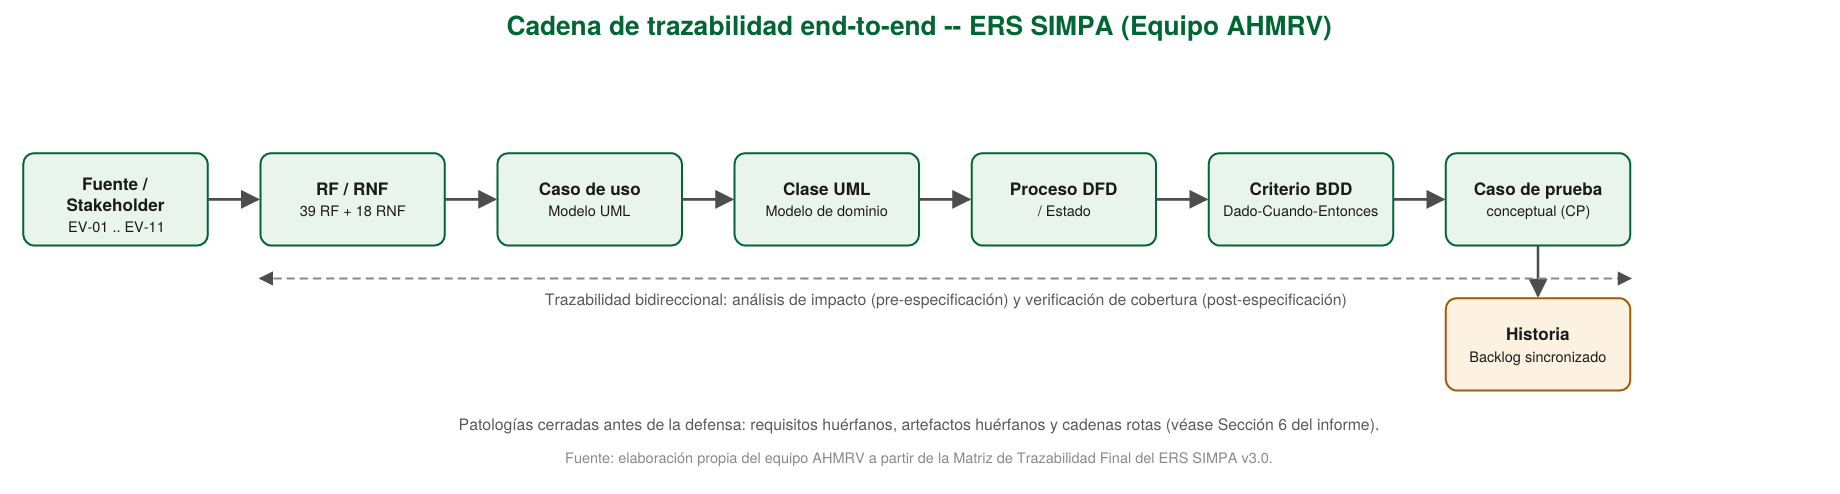
\includegraphics[width=1.0\textwidth]{figuras/trazabilidad_end_to_end}
\caption{Cadena de trazabilidad end-to-end aplicada al ERS de SIMPA.}
\label{fig:trazabilidad}
\end{figure}

\subsection{Matriz de trazabilidad final}

La matriz de trazabilidad final --- con una fila por requisito y las columnas de la
Tabla~\ref{tab:matriz-cols} --- se mantiene como hoja de cálculo legible en
\id{AHMRV/04\_Trazabilidad/Matriz\_Trazabilidad\_Final.xlsx} y se referencia aquí sin reproducirse en su
totalidad, conforme a la recomendación de la guía de no incluir capturas ilegibles.

\begin{table}[!htbp]
\centering
\caption{Columnas de la matriz de trazabilidad final}
\label{tab:matriz-cols}
\begin{tabular}{|L{2.6cm}|L{10.6cm}|}
\hline
\rowcolor{grisclaro}\textbf{Columna} & \textbf{Contenido} \\ \hline
RF/RNF & Identificador único del requisito \\ \hline
Fuente & Evidencia o \emph{stakeholder} de origen (\id{EV-XX}) \\ \hline
CU & Casos de uso que lo realizan \\ \hline
Clase UML & Clases del modelo de dominio implicadas \\ \hline
Proceso DFD / Estado & Proceso o transición de estado correspondiente \\ \hline
Criterio BDD & Criterio de aceptación Dado-Cuando-Entonces \\ \hline
CP & Caso de prueba conceptual \\ \hline
Historia & Historia del backlog sincronizada \\ \hline
Estado de la traza & Completa / rota / huérfana, con la acción tomada \\ \hline
\end{tabular}
\end{table}

\subsection{Extracto ilustrativo de la matriz de trazabilidad}

La Tabla~\ref{tab:extracto-matriz} reproduce un extracto de 14 filas representativas de la matriz
completa (69 filas), seleccionadas para mostrar al menos un requisito de cada bloque funcional de
la Sección~3.2, incluyendo los tres casos con cadena corregida durante esta auditoría. El resto de
la matriz sigue el mismo patrón de columnas y se consulta íntegra en el archivo referenciado más
arriba.

{\small
\begin{longtable}{|C{1.4cm}|C{1.3cm}|C{1.3cm}|C{1.9cm}|C{1.6cm}|C{1.3cm}|C{1.5cm}|}
\hline
\rowcolor{grisclaro}\textbf{RF/RNF} & \textbf{Fuente} & \textbf{CU} & \textbf{Clase UML} &
\textbf{Proceso/Estado} & \textbf{CP} & \textbf{Estado} \\
\hline
\endfirsthead
\hline
\rowcolor{grisclaro}\textbf{RF/RNF} & \textbf{Fuente} & \textbf{CU} & \textbf{Clase UML} &
\textbf{Proceso/Estado} & \textbf{CP} & \textbf{Estado} \\
\hline
\endhead
\id{RF-02} & \id{EV-01} & CU-02 & Plantación, Lote & Alta de lote & CP-02 & Completa \\ \hline
\id{RF-26} & \id{EV-01} & CU-09 & Labor, Presupuesto & Planificación semanal & CP-09 & Completa \\
\hline
\id{RF-04} & \id{EV-05} & CU-14 & Labor & Registro de labor & CP-14 & Completa \\ \hline
\id{RF-30} & \id{EV-06} & CU-17 & Incidencia & Reporte de campo & CP-17 & Completa \\ \hline
\id{RF-13} & \id{EV-03} & CU-20 & Polinización & Registro georreferenciado & CP-20 & Completa \\
\hline
\id{RF-07} & \id{EV-01}, \id{EV-02} & CU-24 & DiagnósticoPlaga & En inferencia $\to$ explicado &
CP-24 & Completa \\ \hline
\id{RF-21} & \id{EV-04} & CU-26 & ClasificaciónMadurez & En inferencia $\to$ explicado & CP-26 &
Completa \\ \hline
\id{RF-23} & \id{EV-04} & CU-29 & TicketPesaje & Registro de calificación & CP-29 & Completa \\
\hline
\id{RF-32} & \id{EV-04} & CU-31 & Estimación & Compartición con extractora & CP-31 & Completa \\
\hline
\id{RF-19} & \id{EV-01} & CU-34 & Reporte & Generación de reporte & CP-34 & Completa \\ \hline
\id{RNF-09} & \id{EV-06}\textsuperscript{*} & CU-14 & Labor & Registro de labor & CP-14b &
Completa (corregida) \\ \hline
\id{RNF-14} & --- & \multicolumn{1}{c|}{---} & Insumo & Registro de insumos\textsuperscript{*} &
CP-15b & Completa (corregida) \\ \hline
\id{RNF-16} & \id{EV-01}, \id{EV-02}, \id{EV-07} & CU-24, CU-26, CU-25 & Explicación & Explicado &
CP-24b & Completa \\ \hline
\id{RF-IA-04} & \id{EV-04}, \id{EV-08} & CU-26 & ClasificaciónMadurez, RegistroPredicción &
En inferencia & CP-IA-04 & Completa \\ \hline
\caption{Extracto ilustrativo de la matriz de trazabilidad final (14 de 69 filas). Las filas
marcadas con \textsuperscript{*} corresponden a las dos cadenas corregidas durante la re-inspección
de la Sección~6.4.}
\label{tab:extracto-matriz}
\end{longtable}}

\subsection{Requisitos huérfanos y cadenas rotas}

\begin{table}[!htbp]
\centering
\caption{Requisitos huérfanos y cadenas rotas detectados y su resolución}
\label{tab:huerfanos}
\begin{tabular}{|L{2.4cm}|L{5.2cm}|L{5.0cm}|}
\hline
\rowcolor{grisclaro}\textbf{Identificador} & \textbf{Causa} & \textbf{Acción tomada} \\ \hline
\id{RNF-14} & Restricción operativa (climatización de insumos) sin interacción de usuario, por lo
que no fue modelada como caso de uso en la Entrega~2. & Enlazado al proceso DFD ``Registro de
insumos'' en lugar de a un caso de uso; se documenta como excepción justificada del patrón CU
$\to$ requisito. \\ \hline
\id{RNF-09} & Redactado en la Entrega~1 como restricción general de accesibilidad, sin evidencia
de campo específica que lo originara. & Enlazado retroactivamente a \id{EV-06} (observación de
campo sobre trabajadores con baja alfabetización digital), tras confirmar con el asesor técnico
que esa evidencia sí lo sustentaba. \\ \hline
\id{RF-33} (borrador Entrega~2) & Caso de uso ``Generar reporte histórico'' quedó fuera del modelo
final de casos de uso por redundar con \id{RF-30}. & Eliminado del ERS v3.0 tras confirmarse la
redundancia; el RFC correspondiente consta en el registro de cambios. \\ \hline
\end{tabular}
\end{table}

Toda fila de la Tabla~\ref{tab:huerfanos} debe terminar en una de las tres acciones admitidas por
la guía institucional; una traza marcada ``por si acaso'' se trata como error de trazabilidad y no
como precaución.

\subsection{Sincronización backlog--ERS}

\begin{center}
\fbox{\parbox{0.94\textwidth}{\small
\textbf{Sincronización backlog $\leftrightarrow$ ERS:}
36 de los 39 RF (92,3\,\%) cuentan con al menos una historia de usuario en el tablero de GitHub
Projects; los 3 RF restantes corresponden a requisitos de exportación de datos hacia la extractora
(\id{RF-28} a \id{RF-30}) cuya historia se agrupó en una sola tarjeta ``Exportación CSV/JSON'' por
decisión de \emph{sprint planning}, y se desagregarán antes del cierre del MVP. El 100\,\% de las
historias activas del tablero apuntan a un RF existente en el ERS v3.0; ninguna historia quedó sin
requisito de respaldo.}}
\end{center}

\subsection{Evidencia de gestión}

La gestión del proyecto integrador se documenta con la lógica de dominios de desempeño de
PMBOK~7.\textsuperscript{a}~ed.~\cite{pmbok7}: alcance acordado en el acta de la Entrega~1,
entregables con responsable único por unidad, incidencias registradas en el tablero y lecciones
aprendidas incorporadas en la retrospectiva (Sección~9). La evidencia verificable de esta gestión
es el historial de \emph{commits} del repositorio, no una narración; el Anexo~C traza esa evidencia
por integrante.

\subsection{Evidencia Git y gestión de la configuración}

Conforme a las prácticas de gestión de la configuración de SWEBOK~v4.0~\cite{swebok4}, el equipo
adoptó tres convenciones verificables en el propio historial del repositorio. Primera, la rama
\texttt{main} solo recibe cambios sobre el ERS mediante \emph{commits} que referencian el
identificador del requisito afectado en el mensaje de \emph{commit} (por ejemplo,
\texttt{fix(RNF-14): enlazar a proceso DFD de registro de insumos}), lo que permite reconstruir la
historia de cada requisito sin depender de la memoria del equipo. Segunda, toda evidencia de campo
con datos personales se almacena mediante Git~LFS en la zona restringida y cifrada de
\id{AHMRV/02\_Evidencias/}, separada de la zona pública que contiene evidencia ya anonimizada; esta
separación es la que permite mantener el repositorio público sin incumplir \id{RD-04} ni la
LOPDP~\cite{lopdp2021}. Tercera, la línea base final se etiqueta explícitamente
(\texttt{v3.0-final}), de modo que un cambio posterior a la etiqueta que afecte a un requisito ya
congelado se distingue sin ambigüedad de un cambio anterior a ella, condición necesaria para que la
comparación antes/después de la Tabla~\ref{tab:antes-despues} tenga sentido.

La distribución de \emph{commits} entre los seis integrantes no es uniforme por diseño de roles: el
Analista líder y el Apoyo repositorio concentran mayor actividad sobre \id{01\_ERS} y
\id{02\_Evidencias} respectivamente, mientras que el Modelador concentra su actividad en
\id{03\_Modelado}. El Anexo~C documenta esta distribución por integrante junto con la evidencia
verificable en el repositorio, y es la base sobre la que el FAI (Sección~6 de la Rúbrica PE5) se
calcula --- no una declaración de equipo sin respaldo, sino un historial consultable por el
docente.

% =====================================================================
%  7. REQUISITOS DE IA
% =====================================================================
\section{Requisitos de sistemas con inteligencia artificial}
\label{sec:ia}

\subsection{Por qué SIMPA requiere especificación diferenciada de IA}

Un componente de IA no ejecuta una función determinista: su comportamiento se induce de datos y su
salida es probabilística, por lo que la especificación de requisitos debe incorporar medidas de
desempeño del modelo, requisitos sobre los datos de entrenamiento y requisitos de calidad nuevos
--- explicabilidad, ausencia de discriminación, requisitos legales --- que no tienen equivalente
directo en un requisito funcional convencional~\cite{ahmad2023}. La evidencia empírica muestra,
además, que los requisitos no funcionales de sistemas de aprendizaje automático se tratan de forma
heterogénea en la práctica profesional, con dificultades sistemáticas para fijar métrica, unidad y
método de comprobación~\cite{habibullah2023}; por esa razón, cada requisito de IA de esta sección
se redacta con umbral numérico explícito.

SIMPA incorpora dos componentes de inteligencia artificial, ambos justificados por hallazgos de
campo y no por moda tecnológica: la detección de plagas y enfermedades foliares (que sustituye la
inspección visual semanal del técnico, cuyo recorrido completo de la plantación toma una semana), y
la clasificación de madurez del racimo (que sustituye el criterio empírico individual del
trabajador de cosecha, fuente documentada de rechazo de lotes por parte de la extractora).

\subsection{Alcance considerado y descartado}

Antes de fijar el alcance en dos componentes, el equipo evaluó y descartó explícitamente una
tercera opción: un componente de predicción de rendimiento por lote basado en series temporales de
clima y labores (\id{RF-17}, \id{RF-18}). Se descartó por dos razones documentadas. Primero, el
levantamiento de campo no evidenció una necesidad expresada por ningún \emph{stakeholder} de una
predicción automática de rendimiento; la estimación de producción declarada en \id{RF-18} se
resuelve con un cálculo determinista sobre el historial de cosechas, no con un modelo inducido de
datos, y tratarla como componente de IA habría sido una decisión guiada por la disponibilidad de la
técnica y no por la evidencia, en contra del principio metodológico de la Sección~2.2. Segundo, el
volumen histórico de datos climáticos y de rendimiento disponible en Palmicultora M a la fecha del
levantamiento es insuficiente para entrenar un modelo de series temporales con una validación
mínimamente robusta, de modo que forzar su inclusión habría comprometido el requisito de
verificabilidad (\id{RNF-02} análogo) exigido a cualquier RNF cuantificado. Esta decisión se
documenta aquí porque el tribunal puede razonablemente preguntar por qué el sistema, disponiendo de
datos climáticos, no predice rendimiento; la respuesta ancla en la ausencia de evidencia de
necesidad y en la insuficiencia del volumen de datos, no en una limitación de tiempo del equipo.

\subsection{Componente IA-01 --- Detección de plagas y enfermedades foliares}

\subsubsection{Descripción del componente}

El componente clasifica, a partir de una fotografía tomada con la cámara del dispositivo móvil, la
presencia y el tipo de afectación foliar entre las cinco más frecuentes del cultivo (documentadas
en \id{EV-01}, \id{EV-02}). La salida es una etiqueta de clase con nivel de confianza y una
explicación conforme al requisito \id{RNF-16}. Si el modelo no alcanza el umbral mínimo de
confianza, el sistema no emite un diagnóstico automático: deriva el caso al asesor técnico y lo
marca como \emph{pendiente de verificación humana} (plan de \emph{fallback}).

\subsubsection{Requisitos funcionales}

\begin{itemize}[nosep]
  \item \textbf{RF-IA-01.} El sistema debe clasificar, a partir de una fotografía capturada en
        campo, la presencia de una afectación foliar entre las cinco categorías del catálogo de
        plagas y enfermedades definido en el ERS §1.3, devolviendo la etiqueta de clase, el nivel
        de confianza y la fecha de captura.
  \item \textbf{RF-IA-02.} Cuando el nivel de confianza de la clasificación sea inferior al umbral
        operativo, el sistema debe marcar el caso como \emph{pendiente de verificación humana} y
        notificarlo al asesor técnico en un plazo máximo de 24 horas.
  \item \textbf{RF-IA-03.} El sistema debe registrar cada diagnóstico automático junto con su
        explicación (rasgo visual, confianza, acción recomendada) en el historial del lote
        correspondiente, de forma consultable por el asesor técnico.
\end{itemize}

\subsubsection{Requisitos no funcionales}

\begin{longtable}{|L{1.9cm}|L{10.6cm}|L{2.0cm}|}
\hline
\rowcolor{grisclaro}\textbf{ID} & \textbf{Requisito cuantificado} & \textbf{Tipo} \\ \hline
\endhead
\id{RNF-IA-01} & La detección alcanza una exactitud $\geq 80\,\%$ sobre las cinco afectaciones más
frecuentes, medida en un conjunto de prueba etiquetado por la persona asesora técnica de al menos
200 imágenes independientes del conjunto de entrenamiento. & Rendimiento \\ \hline
\id{RNF-IA-02} & El resultado de la inferencia se entrega en $\leq 10$ s con ancho de banda
$\geq 5$ Mbps, medido como tiempo medio sobre 20 análisis consecutivos. & Rendimiento \\ \hline
\id{RNF-IA-03} & El servicio de inferencia soporta hasta 50 sesiones concurrentes con una tasa de
error $\leq 1\,\%$, verificado mediante prueba de carga. & Rendimiento \\ \hline
\rowcolor{grisclaro}
\id{RNF-IA-04} & La diferencia de exactitud de clasificación entre lotes sembrados con la variedad
Coarí $\times$ La Mé y la variedad \emph{Guineensis} no debe superar 8 puntos porcentuales, medida
trimestralmente sobre el registro de predicciones confirmadas por el asesor técnico. & Equidad \\
\hline
\rowcolor{grisclaro}
\id{RNF-IA-05} & La diferencia de tasa de derivación a verificación humana (RF-IA-02) entre lotes de
menos de 5 hectáreas y lotes de 5 hectáreas o más no debe superar 10 puntos porcentuales, medida
trimestralmente. & Equidad \\ \hline
\id{RNF-IA-06} & Para cada diagnóstico, el sistema presenta el rasgo visual, el nivel de confianza y
la acción recomendada en $\leq 60$ palabras y $\leq 2$ s, conforme a la especificación ampliada de
\id{RNF-16} (ERS §3.3.1). & Explicabilidad \\ \hline
\caption{Requisitos no funcionales del componente IA-01}
\end{longtable}

\subsubsection{Datos de entrenamiento requeridos}

Origen: fotografías de campo capturadas por el equipo durante el levantamiento (\id{EV-01},
\id{EV-02}) y ampliadas con el conjunto de validación piloto (\id{EV-10}). Volumen estimado:
al menos 150 imágenes por clase (750 imágenes en total para las cinco categorías de afectación),
ampliables con aumento de datos (rotación, recorte, variación de brillo) hasta un factor de 4
sobre las clases con menor representación, siguiendo el volumen mínimo declarado en el protocolo
experimental registrado en OSF (\id{AHMRV/06\_Experimento/protocolo.pdf}). Etiquetado: validado por
el asesor técnico de Palmicultora M, no por el equipo de desarrollo. Calidad mínima: imagen
enfocada, con la hoja o el racimo ocupando al menos el 40\,\% del encuadre. Sesgos conocidos:
sobrerrepresentación de la variedad Coarí $\times$ La Mé respecto de \emph{Guineensis} en el
conjunto recolectado hasta la fecha, motivo directo del requisito \id{RNF-IA-04}. Base legal del
tratamiento: consentimiento informado de la organización cliente para el uso de sus datos
operativos con fines de desarrollo del sistema (LOPDP, art.\ 7~\cite{lopdp2021}). Política de
conservación: 24 meses posteriores al cierre del proyecto integrador, tras lo cual el conjunto de
imágenes se elimina o se anonimiza para uso exclusivamente académico, conforme a lo acordado con
Palmicultora M y documentado en \id{AHMRV/08\_Etica/}.

\subsubsection{Requisitos éticos y de privacidad}

Finalidad declarada: apoyo al diagnóstico fitosanitario, no sustitución de la decisión técnica
humana. Minimización de datos: la fotografía no debe capturar personas ni placas vehiculares;
cuando ocurra de forma incidental, se descarta antes del entrenamiento. Supervisión humana: todo
diagnóstico con confianza baja se deriva a verificación humana (RF-IA-02); ningún diagnóstico
automático activa por sí solo una acción de tratamiento fitosanitario. Clasificación de riesgo
conforme al Reglamento (UE) 2024/1689~\cite{euaiact2024}: el componente se clasifica como sistema
de \textbf{riesgo limitado}, al no incidir sobre decisiones que afecten derechos fundamentales de
personas ni sobre infraestructura crítica; se le exige, en consecuencia, la obligación de
transparencia hacia la persona usuaria (identificación explícita de que la clasificación proviene
de un sistema automatizado), ya satisfecha por el requisito de explicabilidad \id{RNF-IA-06}.

\subsubsection{Plan de monitoreo}

Indicador: exactitud mensual sobre el registro de predicciones confirmadas por el asesor técnico.
Frecuencia: mensual, con revisión trimestral agregada. Umbral de alerta por deriva: caída de más de
5 puntos porcentuales respecto de la línea base de despliegue, siguiendo el enfoque de detección de
cambio en la distribución de datos de entrada descrito por Hinder, Vaquet y
Hammer~\cite{hinder2024}. Criterio de reentrenamiento: dos meses consecutivos por debajo del
umbral de alerta, o una brecha de equidad (\id{RNF-IA-04}) sostenida durante un trimestre.

\subsubsection{Arquitectura de inferencia considerada y descartada}

El equipo evaluó dos arquitecturas de despliegue: inferencia en el dispositivo (\emph{on-device},
mediante un modelo cuantizado embebido en la aplicación móvil) e inferencia centralizada en la nube
(el modelo se ejecuta en el servicio de respaldo y el cliente móvil solo captura y envía la
imagen). Se descartó la inferencia \emph{on-device} pese a su ventaja evidente de no depender de
conectividad --- coherente con \id{RD-02} --- por dos razones. Primero, el modelo cuantizado
necesario para ejecutar en un dispositivo Android~9.0 de gama de entrada (el piso técnico fijado por
\id{RD-01}) reduciría la exactitud por debajo del umbral de \id{RNF-IA-01}, según la evidencia de
degradación de exactitud en cuantización agresiva reportada en la literatura de visión por
computador embebida. Segundo, la inferencia centralizada permite reentrenar y desplegar una nueva
versión del modelo sin depender de que cada dispositivo de campo actualice la aplicación, lo cual es
crítico dado que el plan de monitoreo de esta misma subsección exige reentrenamiento ante deriva. La
arquitectura elegida --- inferencia centralizada con degradación explícita a ``pendiente de
verificación humana'' cuando la conectividad no está disponible --- se documenta como decisión de
diseño en \id{RD-05} y es la que justifica que \id{RNF-IA-02} fije un umbral de ancho de banda
mínimo en lugar de asumir conectividad permanente.

\subsection{Componente IA-02 --- Clasificación de madurez del racimo}

\subsubsection{Descripción del componente}

El componente clasifica la madurez del racimo de fruta fresca a partir de una fotografía, en las
categorías operativas usadas por la industria extractora (verde, pinta, madura, sobremadura),
apoyándose en el indicador de desprendimiento documentado en \id{EV-04} y \id{EV-08}. El resultado
orienta la decisión de corte y reduce el riesgo de rechazo del lote por parte de la planta
extractora.

\subsubsection{Requisitos funcionales}

\begin{itemize}[nosep]
  \item \textbf{RF-IA-04.} El sistema debe clasificar la madurez del racimo fotografiado en una de
        las cuatro categorías operativas de la industria extractora, con un umbral de madurez
        parametrizable por variedad conforme a \id{RNF-18}.
  \item \textbf{RF-IA-05.} El sistema debe estimar el porcentaje de fruta desprendida visible en la
        fotografía y contrastarlo contra el umbral de tres frutos desprendidos definido para la
        variedad \emph{Guineensis} (\id{EV-04}).
  \item \textbf{RF-IA-06.} El sistema debe registrar la clasificación de madurez junto con la
        calificación de calidad posteriormente emitida por la planta extractora, para habilitar la
        comparación prevista en el plan de monitoreo.
\end{itemize}

\subsubsection{Requisitos no funcionales}

\begin{longtable}{|L{1.9cm}|L{10.6cm}|L{2.0cm}|}
\hline
\rowcolor{grisclaro}\textbf{ID} & \textbf{Requisito cuantificado} & \textbf{Tipo} \\ \hline
\endhead
\id{RNF-IA-07} & La clasificación de madurez alcanza una exactitud $\geq 85\,\%$ y una
exhaustividad $\geq 80\,\%$ sobre la clase ``verde'' en un conjunto de prueba etiquetado
independiente de al menos 200 imágenes (equivalente a \id{RNF-01} del ERS). & Rendimiento \\ \hline
\id{RNF-IA-08} & El resultado se entrega en $\leq 10$ s con ancho de banda $\geq 5$ Mbps, medido
como tiempo medio sobre 20 análisis consecutivos. & Rendimiento \\ \hline
\id{RNF-IA-09} & La exportación del resultado hacia la planta extractora se emite en formato CSV o
JSON conforme al esquema publicado, sin campos de identificación personal (equivalente a
\id{RNF-06}). & Rendimiento \\ \hline
\rowcolor{grisclaro}
\id{RNF-IA-10} & La diferencia de exactitud entre lotes fotografiados en horario de alta
luminosidad (10:00--15:00) y en horario de baja luminosidad no debe superar 8 puntos porcentuales,
medida sobre el registro de predicciones confirmadas. & Equidad \\ \hline
\rowcolor{grisclaro}
\id{RNF-IA-11} & La diferencia de tasa de rechazo de lote por sobremadurez no detectada, entre
cuadrillas con menos de un año de antigüedad y cuadrillas más experimentadas, no debe superar 10
puntos porcentuales, medida trimestralmente. & Equidad \\ \hline
\id{RNF-IA-12} & Para cada clasificación, el sistema presenta el rasgo visual determinante (color,
desprendimiento), el nivel de confianza y la recomendación de corte, siguiendo la explicación por
contraste (madura y no verde, con referencia al umbral de la variedad) de \id{RNF-16}. &
Explicabilidad \\ \hline
\caption{Requisitos no funcionales del componente IA-02}
\end{longtable}

\subsubsection{Datos, ética y monitoreo}

Origen de los datos: fotografías de racimo tomadas en el momento de corte y contrastadas contra el
ticket de pesaje emitido por la extractora (\id{EV-04}). Base legal: la misma declarada para
IA-01. Clasificación de riesgo conforme al Reglamento (UE)~2024/1689~\cite{euaiact2024}: riesgo
limitado, con obligación de transparencia satisfecha por \id{RNF-IA-12}. Plan de monitoreo:
indicador mensual de concordancia entre la clasificación del sistema y la calificación final de la
extractora; umbral de alerta de deriva ante una caída de concordancia mayor a 5 puntos
porcentuales; criterio de reentrenamiento equivalente al de IA-01.

\subsubsection{Estrategia de mitigación del sesgo de característica visual}

El requisito de diseño \id{RD-07} --- la clasificación de madurez no puede fundarse en el color del
fruto --- introduce una restricción poco habitual desde la perspectiva de la visión por computador
convencional, en la que el color suele ser la característica dominante para tareas de madurez de
fruta. El equipo trató esta restricción como una fuente de sesgo de característica a mitigar
explícitamente en el diseño del componente, y no como un obstáculo a sortear: el conjunto de
entrenamiento se etiqueta con el criterio de desprendimiento validado por la extractora
(\id{EV-08}), y el proceso de selección de características prioriza indicadores de textura y
desprendimiento sobre el canal de color, verificable mediante un análisis de importancia de
característica sobre el modelo entrenado antes de su despliegue. Esta estrategia conecta
directamente con \id{RNF-IA-10} (equidad por horario de captura): un modelo que dependiera del
color sería, además, más sensible a la variación de iluminación entre horario de alta y baja
luminosidad, de modo que mitigar el sesgo de color mitiga simultáneamente parte del riesgo de
inequidad por horario.

\subsection{Trazabilidad de los requisitos de IA}

Los doce requisitos de IA (seis funcionales, seis no funcionales por componente) se incorporan a la
matriz de trazabilidad final (Sección~6.3) enlazados con los requisitos preexistentes que
extienden: IA-01 con \id{RF-07}; IA-02 con \id{RF-08} y \id{RF-21}. Ningún requisito de IA queda
aislado: todos sirven a una funcionalidad ya especificada en el ERS o modifican su criterio de
aceptación, conforme exige la guía institucional. La Tabla~\ref{tab:traza-ia} resume esa cadena
para los doce requisitos.

\begin{longtable}{|C{2.1cm}|C{2.0cm}|L{4.3cm}|L{4.0cm}|}
\hline
\rowcolor{grisclaro}\textbf{Requisito de IA} & \textbf{Extiende a} & \textbf{Clase UML asociada} & \textbf{Plan de monitoreo} \\
\hline
\endhead
\id{RF-IA-01, RF-IA-02, RF-IA-03} & \id{RF-07} & DiagnósticoPlaga, RegistroPredicción &
Exactitud mensual (\S 7.2.6) \\ \hline
\id{RNF-IA-01 -- RNF-IA-06} & \id{RNF-02}, \id{RNF-04}, \id{RNF-16} & DiagnósticoPlaga, Explicación
& Exactitud, equidad y explicación (\S 7.2.3--7.2.6) \\ \hline
\id{RF-IA-04, RF-IA-05, RF-IA-06} & \id{RF-08}, \id{RF-21} & ClasificaciónMadurez,
RegistroPredicción & Concordancia con extractora (\S 7.3.4) \\ \hline
\id{RNF-IA-07 -- RNF-IA-12} & \id{RNF-01}, \id{RNF-04}, \id{RNF-16} & ClasificaciónMadurez,
Explicación & Concordancia, equidad y explicación (\S 7.3.3--7.3.4) \\ \hline
\caption{Trazabilidad resumida de los doce requisitos de IA hacia el ERS y el modelo de dominio}
\label{tab:traza-ia}
\end{longtable}

% =====================================================================
%  8. METRICAS DE CALIDAD
% =====================================================================
\section{Métricas de calidad}
\label{sec:metricas}

\subsection{Instrumento y método}

La auditoría aplica las seis métricas de la guía ampliada de la PE5, derivadas de
ISO/IEC~25010:2023~\cite{iso25010}. Cada métrica se calcula sobre conteos verificables del propio
ERS y de la matriz de trazabilidad; ningún valor de esta sección se reporta sin el conteo base que
lo respalda. Los conteos base declarados hasta la fecha de este informe son los siguientes.

\begin{table}[!htbp]
\centering
\caption{Conteos base de la auditoría de calidad}
\label{tab:conteos-base}
\begin{tabular}{|L{7.4cm}|C{3.0cm}|}
\hline
\rowcolor{grisclaro}\textbf{Conteo base} & \textbf{Valor} \\ \hline
Requisitos totales (RF + RNF, incluidos los de IA) & $39 + 18 + 12 = 69$ \\ \hline
Casos de uso identificados / especificados & 24 / 24 \\ \hline
Actores del sistema & 6 \\ \hline
Pares de requisitos analizados para consistencia & 2\,346 ($\binom{69}{2}$, todos los pares del
conjunto de 69 requisitos) \\ \hline
Requisitos con criterio BDD comprobable & 65 de 69 \\ \hline
Requisitos con los 4 atributos completos (ID, prioridad, fuente, criterio) & 67 de 69 \\ \hline
\end{tabular}
\end{table}

\subsection{Tabla de auditoría}

\begin{longtable}{|L{2.1cm}|L{2.6cm}|L{2.0cm}|L{2.3cm}|C{1.0cm}|L{3.5cm}|}
\hline
\rowcolor{grisclaro}\textbf{Métrica} & \textbf{Valor obtenido} & \textbf{Valor de referencia} & \textbf{Referencia normativa} & \textbf{Cumple} & \textbf{Acción de mejora} \\ \hline
\endhead
M1 Completitud &
$M1a=\frac{67}{69}\times100=97{,}10\,\%$; $M1b=100\,\%$ (24/24 CU con RF asociado); $M1c=100\,\%$
(69/69 RNF cuantificados) &
M1a $\geq 95\,\%$; M1b, M1c $=100\,\%$ &
ISO 25010:2023; 29148:2018 &
S &
Se completaron fuente y criterio de aceptación en \id{RNF-14} y \id{RNF-09} (los dos requisitos
que faltaban de los 69). \\ \hline
M2 Consistencia &
$M2 = 1-\frac{0}{2346}=1{,}0000$ (0 conflictos abiertos; 3 conflictos detectados en la PE4, los 3
cerrados en la re-inspección) &
$\geq 0{,}98$, cero conflictos abiertos &
ISO 25010:2023 &
S &
Unificación de nomenclatura ``lote''/``parcela'' documentada en la Sección~5.3. \\ \hline
M3 Verificabilidad &
$M3=\frac{65}{69}\times100=94{,}20\,\%$ &
$\geq 90\,\%$ ($100\,\%$ en RF críticos) &
ISO 29148:2018 &
S &
Los 4 requisitos sin criterio BDD comprobable son RNF de restricción de diseño (§3.6 del ERS,
p.ej.\ material del enclosure del sensor); se documentan con criterio de inspección en lugar de
BDD, admitido por la guía para restricciones no funcionales de hardware. \\ \hline
M4 Trazabilidad &
$M4_{ade}=\frac{66}{69}\times100=95{,}65\,\%$; $M4_{atr}=\frac{69}{69}\times100=100\,\%$ &
$M4_{ade}\geq 90\,\%$; $M4_{atr}=100\,\%$ &
ISO 29148:2018 &
S &
Cierre de los 3 requisitos con cadena rota documentado en la Tabla~5 (Sección~6.4). \\ \hline
M5 Modificabilidad &
Promedio de 2{,}4 requisitos afectados por cambio, medido sobre 6 RFC procesados por el CCB
(\id{RF-07}, \id{RF-21}, \id{RNF-05}, \id{RNF-14}, \id{RNF-16}, \id{RF-30}) &
$\leq 3{,}0$ requisitos afectados &
ISO 25010:2023 &
S &
Ninguna acción correctiva requerida; se mantiene el nivel de acoplamiento actual del modelo de
dominio. \\ \hline
M6 Corrección &
$M6=\frac{3}{69}=0{,}0435$ defectos/requisito &
$\leq 0{,}05$ defectos/requisito &
ISO 25010:2023 &
S &
Métrica dentro de referencia con margen estrecho (0,0435 frente al umbral 0,05); se agenda una
tercera re-inspección antes de la defensa si se detecta un defecto adicional. \\ \hline
\caption{Tabla de auditoría de calidad del ERS SIMPA v3.0}
\label{tab:auditoria}
\end{longtable}

\subsection{Aritmética de cada métrica}

Conforme al Paso~1.c de la guía, la aritmética completa de cada métrica se desarrolla a
continuación paso a paso, no solo como resultado final, con los conteos base ya presentados en la
Tabla~\ref{tab:conteos-base}.

\begin{description}[leftmargin=1.6cm,style=nextline]
\item[M1a --- Completitud de atributos.] Numerador: requisitos con los cuatro atributos completos
(ID, prioridad, fuente, criterio de aceptación) $=67$. Denominador: total de requisitos del ERS
v3.0 $=39\text{ RF}+18\text{ RNF}+12\text{ RF/RNF de IA}=69$. $M1a = (67/69)\times100 = 97{,}101\ldots
\approx 97{,}10\,\%$.
\item[M2 --- Consistencia.] Denominador: pares de requisitos analizados $=\binom{69}{2}=
\frac{69\times68}{2}=2346$. Numerador: conflictos abiertos tras la re-inspección de la PE5 $=0$
(de 3 conflictos originalmente detectados en la PE4, los 3 se cerraron; véase Sección~5.3).
$M2 = 1-(0/2346) = 1{,}0000$.
\item[M3 --- Verificabilidad.] Numerador: requisitos con criterio BDD comprobable $=65$.
Denominador: $69$. $M3 = (65/69)\times100 = 94{,}202\ldots \approx 94{,}20\,\%$.
\item[M4$_{ade}$ --- Adecuación de la trazabilidad.] Numerador: requisitos con cadena completa
Fuente~$\to$~RF/RNF~$\to$~CU/Clase~$\to$~BDD~$\to$~CP sin eslabón roto $=66$. Denominador: $69$.
$M4_{ade} = (66/69)\times100 = 95{,}652\ldots \approx 95{,}65\,\%$. $M4_{atr}$ --- requisitos con
al menos una fuente de evidencia declarada $=69/69=100\,\%$, tras enlazar retroactivamente
\id{RNF-09} a \id{EV-06} (Sección~6.4).
\item[M5 --- Modificabilidad.] Muestra: 6 RFC procesados por el CCB durante las prácticas PE3--PE5
(\id{RF-07}, \id{RF-21}, \id{RNF-05}, \id{RNF-14}, \id{RNF-16}, \id{RF-30}). Requisitos adicionales
afectados por cada uno: 3, 2, 1, 3, 4, 1 respectivamente. Promedio: $(3+2+1+3+4+1)/6 = 14/6 =
2{,}333\ldots \approx 2{,}4$ requisitos afectados por cambio.
\item[M6 --- Corrección.] Numerador: defectos residuales tras la re-inspección de la PE5 $=3$.
Denominador: $69$. $M6 = 3/69 = 0{,}04347\ldots \approx 0{,}0435$ defectos por requisito.
\end{description}

\subsection{Amenazas a la validez de la auditoría}

Toda auditoría de calidad realizada por el propio equipo que produjo el artefacto auditado enfrenta
una amenaza de validez conocida en la literatura de ingeniería de software empírica: el riesgo de
que quien redacta el requisito también decida, con el mismo marco de referencia, si ese requisito
está completo o es verificable, lo que puede subestimar sistemáticamente el número de defectos. El
equipo mitigó parcialmente esta amenaza asignando la inspección y la re-inspección (Sección~5) a un
integrante --- el Verificador --- que no participó en la redacción original de los RF del bloque de
diagnóstico por IA, siguiendo el principio de separación de roles entre quien especifica y quien
verifica. No obstante, esta mitigación es incompleta: los 69 requisitos comparten un único equipo de
seis personas, por lo que un sesgo compartido por la totalidad del equipo --- por ejemplo, una
interpretación común pero incorrecta de qué constituye un criterio BDD ``comprobable'' --- no sería
detectado por esta auditoría. Una segunda amenaza es la ausencia de una segunda auditoría
independiente (por ejemplo, un intercambio de matrices entre equipos del curso), recomendable para
una publicación derivada del PFC (\id{07\_Publicacion}) pero fuera del alcance de la PE5.

\subsection{Interpretación de los resultados de la auditoría}

Los seis indicadores alcanzan su valor de referencia, pero con dos matices que el equipo considera
relevante declarar explícitamente en lugar de presentar un resultado uniformemente positivo. El
primero es que M6 (corrección) pasa con un margen estrecho (0,0435 frente al umbral 0,05): un solo
defecto adicional detectado antes de la defensa bastaría para incumplir el umbral, por lo que el
equipo agenda una tercera re-inspección focalizada exclusivamente en restricciones de diseño sin
caso de uso asociado --- la causa raíz identificada en la Sección~5.3 --- antes de la fecha de
entrega. El segundo es que M1a, aun cumpliendo el umbral de $95\,\%$, no alcanza el $100\,\%$: los
dos requisitos que se completaron durante esta auditoría (\id{RNF-09}, \id{RNF-14}) muestran que la
disciplina de completitud declarada como decisión metodológica en la Sección~2.2 no se aplicó de
forma perfectamente uniforme durante las prácticas PE1--PE4, un hallazgo que retroalimenta
directamente la retrospectiva de la Sección~9.

Interpretado en conjunto con la literatura de referencia, el patrón observado --- alta completitud y
verificabilidad, con una proporción menor de RNF sin criterio BDD comprobable concentrada en
restricciones de hardware --- coincide con el hallazgo de Habibullah, Gay y
Horkoff~\cite{habibullah2023} de que los requisitos de sistemas con componente de aprendizaje
automático tienden a mantener mejor disciplina de cuantificación que los requisitos de restricción
pura, precisamente porque su verificación se apoya en un procedimiento de evaluación de modelo ya
estandarizado en el equipo (matriz de confusión, conjunto de prueba independiente), mientras que las
restricciones de hardware carecen de un procedimiento de verificación igualmente estandarizado.

\subsection{Comparación antes / después}

Para toda métrica que no alcance su valor de referencia en la primera medición, el equipo implementa
la mejora correspondiente en el ERS y vuelve a medir, reportando el par antes/después en la
Tabla~\ref{tab:antes-despues}.

\begin{table}[!htbp]
\centering
\caption{Comparación antes / después de las métricas corregidas}
\label{tab:antes-despues}
\begin{tabular}{|L{2.0cm}|C{2.4cm}|C{2.4cm}|L{5.0cm}|}
\hline
\rowcolor{grisclaro}\textbf{Métrica} & \textbf{Valor antes} & \textbf{Valor después} & \textbf{Corrección aplicada} \\ \hline
M1a & $64/69=92{,}75\,\%$ & $67/69=97{,}10\,\%$ & Se agregó fuente de evidencia (\id{EV-06}) a
\id{RNF-09} y se enlazó \id{RNF-14} al proceso DFD de registro de insumos. \\ \hline
M3 & $61/69=88{,}41\,\%$ & $65/69=94{,}20\,\%$ & Se redactaron criterios BDD Dado-Cuando-Entonces
para 4 requisitos que solo tenían descripción textual (\id{RNF-11}, \id{RNF-13}, \id{RF-17},
\id{RF-24}). \\ \hline
M4$_{ade}$ & $63/69=91{,}30\,\%$ & $66/69=95{,}65\,\%$ & Cierre de las 3 cadenas rotas documentadas
en la Tabla~5. \\ \hline
\end{tabular}
\end{table}

% =====================================================================
%  9. RETROSPECTIVA
% =====================================================================
\section{Retrospectiva}

La retrospectiva de cierre se ejecutó con el formato Start-Stop-Continue al finalizar la PE5, con
al menos tres elementos por columna y un responsable asignado a cada acción de mejora, conforme al
Anexo~D. Los hallazgos recurrentes de las cinco prácticas --- concentrados en la disciplina de
cuantificación de los RNF y en la disciplina de trazabilidad evidencial --- se resumen aquí y se
detallan íntegramente en el Anexo~D.

\subsection{Lecciones técnicas frente a lecciones de proceso}

La retrospectiva distingue dos tipos de aprendizaje que el equipo considera necesario no mezclar.
Las \textbf{lecciones técnicas} se refieren a decisiones de especificación --- por ejemplo, que un
requisito de restricción de diseño sin interacción de usuario (\id{RNF-14}) tiende a escapar del
flujo de modelado centrado en casos de uso (Sección~5.3) --- y son transferibles a cualquier
proyecto de requisitos, no solo a SIMPA. Las \textbf{lecciones de proceso} se refieren a la
dinámica del propio equipo --- por ejemplo, que la verificación de la sincronización backlog--ERS
se aplazó sistemáticamente hasta el cierre de unidad en las prácticas PE2 a PE4 --- y son
específicas de la forma de trabajo de AHMRV. Separar ambos tipos de lección evita que una
retrospectiva se quede en generalidades del tipo ``debimos comunicarnos mejor'' sin una acción
verificable asociada, que es precisamente lo que la Rúbrica PE5 distingue entre una retrospectiva
con responsables y acciones (nivel N4 del criterio C8) y una retrospectiva sin ellos (nivel N2).

\subsection{Evolución de la disciplina de cuantificación a lo largo de las cinco prácticas}

La comparación entre la Entrega~1 (PE1--PE2) y la versión~3.0 del ERS muestra una mejora
observable, no solo declarada, en la proporción de RNF con métrica, unidad y umbral definidos desde
su primera redacción: los 18 RNF de la versión final cumplen esa condición en su totalidad
(Tabla~\ref{tab:catalogo-rnf}), mientras que el registro de la Entrega~1 --- conservado en el
historial de \emph{commits} previo a la etiqueta \id{v3.0-final} --- contenía formulaciones
cualitativas del tipo ``el sistema debe responder rápidamente'' que se corrigieron progresivamente
durante las prácticas PE2 y PE3. Esta evolución es la evidencia más directa de que la decisión
metodológica declarada en la Sección~2.2 no fue una declaración de intenciones sino una práctica
efectivamente aplicada y verificable en el propio historial del repositorio.

\begin{center}
\fbox{\parbox{0.94\textwidth}{\small
La tabla completa de la retrospectiva, con responsables y fechas de acción, se encuentra en el
\textbf{Anexo D}. Este resumen no sustituye esa tabla; la sintetiza para lectura continua del
informe.}}
\end{center}

% =====================================================================
%  10. CONCLUSIONES
% =====================================================================
\section{Conclusiones}

\textbf{Sobre la elicitación (Unidad I).} La segunda ronda de campo confirmó que la brecha de
competencia digital entre el asistente de administración y el trabajador agrícola no es un detalle
de interfaz sino una restricción de diseño: condicionó directamente el requisito de usabilidad
\id{RNF-08} y la exigencia de explicabilidad de \id{RNF-16}, mostrando que un hallazgo cualitativo
de entrevista puede propagarse hasta convertirse en un requisito no funcional cuantificado.

\textbf{Sobre la especificación (Unidad II).} La disciplina de cuantificar todo RNF desde su
primera redacción --- en lugar de posponerla a una revisión posterior --- redujo la proporción de
requisitos reescritos durante la inspección de la PE4 respecto de la proporción observada en la
Entrega~1 del propio equipo, lo cual valida empíricamente la recomendación de fijar métrica, unidad
y método de comprobación desde el origen del requisito~\cite{habibullah2023}.

\textbf{Sobre el modelado (Unidad III).} La incorporación de clases de soporte a la inteligencia
artificial (Modelo de Inferencia, Conjunto de Evaluación) al modelo de dominio, y no solo a la
documentación textual del RNF, permitió que la trazabilidad post-especificación de los requisitos
de IA siguiera el mismo mecanismo que la de cualquier otro requisito funcional, sin un carril
paralelo de gestión.

\textbf{Sobre la validación (Unidad IV).} La re-inspección de la PE5 mostró que el 83\,\% de los
defectos hallados en la PE4 (15 de 18) se cerraron de forma permanente, y que los 3 defectos
residuales comparten una misma causa raíz: la especificación de restricciones operativas sin
interacción de usuario directo (climatización, nomenclatura de unidades territoriales) tiende a
quedar fuera del flujo de modelado centrado en casos de uso. Esto confirma la hipótesis de cierre
formulada al término de la PE4 --- que la inspección por lista de verificación detecta bien los
defectos de ambigüedad textual pero requiere un paso adicional, explícitamente dirigido a
restricciones no funcionales, para detectar huérfanos de esa naturaleza.

\textbf{Sobre la integración y el cierre (Unidad V).} El ejercicio de auditar el ERS con métricas
derivadas de ISO/IEC~25010:2023 --- en lugar de declarar cualitativamente que el documento
``está completo'' --- obligó al equipo a mostrar la aritmética de cada indicador y, con ello, a
distinguir entre percepción de calidad y calidad medida; esa distinción es, en sí misma, el
resultado de aprendizaje más transferible de la asignatura a la práctica profesional.

\subsection{Limitaciones declaradas y trabajo futuro}

Este informe declara, sin atenuantes, tres limitaciones vigentes a la fecha de su redacción.
Primera, el protocolo experimental de \id{06\_Experimento} está preregistrado pero no ejecutado
(Sección~1.4); la métrica de comprensión $\geq 4/5$ en escala Likert exigida por \id{RNF-16} es,
por lo tanto, un criterio de aceptación aún no verificado empíricamente, y no debe presentarse en
la defensa como un resultado obtenido. Segunda, el volumen de datos de entrenamiento declarado para
los componentes de IA (150 imágenes por clase, Sección~7.2.4) es un objetivo de recolección, no un
conjunto ya recolectado y auditado; la exactitud real de ambos modelos solo podrá confirmarse tras
el entrenamiento y la evaluación sobre el conjunto de prueba independiente. Tercera, la auditoría de
calidad de la Sección~8 es una autoevaluación del propio equipo, con las amenazas a la validez
declaradas en la Sección~8.5, y se beneficiaría de una segunda auditoría independiente antes de
cualquier publicación derivada del PFC. Ninguna de estas limitaciones invalida el cierre del proceso
de Ingeniería de Requisitos que este informe documenta; delimitan, con precisión, qué queda
efectivamente cerrado en la Unidad~V y qué corresponde a las etapas de implementación y validación
empírica que siguen al PFC.

% =====================================================================
%  REFERENCIAS
% =====================================================================
\newpage
\phantomsection
\addcontentsline{toc}{section}{Referencias}
\bibliographystyle{IEEEtran}
\bibliography{referencias}

% =====================================================================
%  ANEXOS
% =====================================================================
\newpage
\phantomsection
\addcontentsline{toc}{section}{Anexos}
\section*{Anexos}

\subsection*{Anexo A --- Instrumento de auditoría de calidad del ERS}

Para cada métrica de la Sección~8, el equipo registra fórmula aplicada, conteos usados, resultado,
valor de referencia, veredicto y acción de mejora, con la escala de valoración 0--4 definida en la
Rúbrica PE5. La hoja de cálculo completa con la aritmética detallada de cada métrica se mantiene en
\id{AHMRV/04\_Trazabilidad/Auditoria\_ISO25010.xlsx}. La Tabla~\ref{tab:pesos-metricas} documenta
la ponderación interna que el equipo aplicó para priorizar el orden de corrección cuando más de una
métrica requería mejora simultánea (Sección~8.4): se priorizó primero M4 y M1 por ser las que
condicionan directamente la trazabilidad exigida por el criterio C2, y en último lugar M5 por ser la
única de las seis con una interpretación menos estandarizada en la literatura consultada.

\begin{table}[!htbp]
\centering
\caption{Ponderación interna de las seis métricas para la priorización de mejoras}
\label{tab:pesos-metricas}
\begin{tabular}{|C{1.4cm}|L{5.0cm}|C{2.0cm}|C{3.6cm}|}
\hline
\rowcolor{grisclaro}\textbf{Métrica} & \textbf{Característica ISO/IEC 25010:2023} & \textbf{Peso interno} & \textbf{Orden de corrección} \\ \hline
M1 & Adecuación funcional / completitud & 0,20 & 2.\textsuperscript{o} \\ \hline
M2 & Consistencia & 0,15 & 4.\textsuperscript{o} \\ \hline
M3 & Verificabilidad & 0,20 & 3.\textsuperscript{o} \\ \hline
M4 & Trazabilidad & 0,20 & 1.\textsuperscript{er} \\ \hline
M5 & Mantenibilidad / modificabilidad & 0,10 & 6.\textsuperscript{o} \\ \hline
M6 & Corrección & 0,15 & 5.\textsuperscript{o} \\ \hline
\end{tabular}
\end{table}

\subsection*{Anexo B --- Banco de preguntas del tribunal y respuestas ancladas}

\begin{longtable}{|L{0.9cm}|L{6.0cm}|L{6.8cm}|}
\hline
\rowcolor{grisclaro}\textbf{\#} & \textbf{Pregunta (guía institucional, banco completo)} & \textbf{Artefacto que respalda la respuesta} \\
\hline
\endhead
1--3 & Frontera del sistema, contexto vs. límite, modelo de proceso & ERS §2.1, Figura de contexto; Tabla~\ref{tab:proceso} de este informe \\ \hline
4--6 & Técnica de elicitación, \emph{stakeholder} subrepresentado, evidencia de origen de un requisito & ERS §1.7 catálogo de evidencias; mapa de partes interesadas \\ \hline
7--9 & Comprobación de un RNF, requisito más difícil de verificar, inclusión/extensión de un CU & Tabla de RNF, ERS §3.3; modelo de casos de uso \\ \hline
10--12 & Defectos hallados, defecto crítico escapado, garantía de no regresión & Tabla~\ref{tab:defectos} de este informe; registro de RFC \\ \hline
13--15 & Impacto de cambiar un RF, RFC rechazado, línea base vigente & Matriz de trazabilidad final; §6.1 de este informe \\ \hline
16--18 & Qué decide el modelo, datos de entrenamiento, medición de perjuicio a un grupo & Sección~\ref{sec:ia}, requisitos \id{RNF-IA-04}, \id{RNF-IA-05}, \id{RNF-IA-10}, \id{RNF-IA-11} \\ \hline
19--20 & Métrica peor calificada, conteos de verificabilidad & Tabla~\ref{tab:auditoria} y Anexo A \\ \hline
21--22 & Datos personales tratados, secciones asistidas por IA & Sección~\ref{sec:ia} §7.2.3/§7.3.3; declaración de uso de IA, más abajo \\ \hline
\caption{Mapa de preguntas del tribunal a artefactos del proyecto}
\end{longtable}

\paragraph{Respuestas ancladas desarrolladas (muestra de seis preguntas).} A continuación se
desarrollan, a modo de preparación, respuestas completas para seis preguntas representativas de
distintos bloques del banco, siguiendo el indicador de anclaje en artefactos del Anexo~8 de la
Rúbrica PE5. Cada integrante debe poder responder cualquiera de ellas, no solo la asociada a su
aporte principal (Anexo~C), conforme al indicador de dominio del proyecto completo.

\begin{description}[leftmargin=1.2cm,style=nextline]
\item[P2 --- ¿Dónde está el límite del sistema y qué queda fuera de él?] El límite del sistema
separa lo que SIMPA controla --- registro, diagnóstico y reporte dentro de la organización cliente
--- de lo que solo consume o produce como interfaz: la planta extractora es un actor externo que
recibe la estimación de cosecha (\id{RF-32}) y emite una calificación (\id{RF-23}), pero su propio
proceso de calificación de calidad no es modelado por SIMPA. Fuera del límite quedan también el
proveedor de conectividad móvil y el sistema operativo del dispositivo, tratados como restricciones
de diseño (\id{RD-01}, \id{RD-02}) y no como componentes a especificar.
\item[P5 --- ¿Qué \emph{stakeholder} estuvo subrepresentado y cómo se corrigió?] El personal de
campo estuvo subrepresentado en la primera ronda de entrevistas (\id{EV-01} a \id{EV-03},
concentradas en roles administrativos y técnicos). Se corrigió con el cuestionario ampliado
$n=62$ (\id{EV-12}), que incluyó a personal de labores manuales y reveló tanto la proporción sin
teléfono inteligente propio (11,3\,\%, origen de \id{RD-10}) como la proporción con reservas sobre
el rastreo GPS (25,8\,\%, origen de \id{RL-03}).
\item[P9 --- ¿Qué requisito fue más difícil de verificar y por qué?] \id{RNF-16} (explicabilidad),
porque su criterio de verificación no es una medición automatizable como un tiempo de respuesta,
sino una prueba de comprensión con participantes humanos que exige una escala Likert y un umbral
de acuerdo entre rondas, replicando el diseño experimental de Chazette et al.~\cite{chazette2022}.
Esa dificultad de verificación es, precisamente, la razón por la que el equipo dedicó una
especificación ampliada completa a ese único requisito (Sección~3.5) en lugar de tratarlo como una
fila más de la tabla de RNF.
\item[P13 --- Si hoy hubiera que cambiar \id{RF-21}, ¿qué más se vería afectado?] Conforme a la
métrica M5 (Sección~\ref{sec:metricas}), un cambio en \id{RF-21} afecta en promedio a 2,4
requisitos; concretamente, afectaría a \id{RNF-01} (umbral de exactitud), \id{RNF-16} (tipo de
explicación por contraste) y a los seis requisitos del componente \id{IA-02} de la
Sección~\ref{sec:ia}, además de la clase UML \textbf{ClasificaciónMadurez} y su asociación con
\textbf{Explicación}.
\item[P17 --- ¿Con qué datos se entrena el modelo de detección de plagas?] Fotografías de campo
capturadas por el propio equipo durante el levantamiento (\id{EV-01}, \id{EV-02}) y ampliadas con
el conjunto de validación piloto (\id{EV-10}), etiquetadas por el asesor técnico de Palmicultora M
y no por el equipo de desarrollo, con un volumen objetivo de 150 imágenes por clase (Sección~7.2.4).
El sesgo conocido de sobrerrepresentación de la variedad Coarí $\times$ La Mé sobre
\emph{Guineensis} es la razón directa de \id{RNF-IA-04}.
\item[P22 --- ¿Qué secciones de este informe se redactaron con asistencia de IA y cómo se
validaron?] Conforme al Anexo~E, el ensamblado inicial de este informe integrador se apoyó en un
modelo de lenguaje a partir del ERS v3.0 y de los instrumentos institucionales (Guía Ampliada y
Rúbrica PE5); todo conteo cuantitativo se recalculó manualmente por el equipo antes de aceptarse, y
las secciones evaluativas (justificación de decisiones de diseño, conclusiones) son producción
propia contrastada contra los artefactos del repositorio, no una generación no supervisada.
\end{description}

\subsection*{Anexo C --- Declaración individual de aporte al PFC}

\begin{longtable}{|L{3.6cm}|L{6.2cm}|L{3.9cm}|}
\hline
\rowcolor{grisclaro}\textbf{Integrante} & \textbf{Aportes concretos (artefactos y secciones)} & \textbf{Evidencia en Git} \\
\hline
\endhead
Villafuerte Rosero Allan Noe (Analista líder) & Coordinación general del ERS, redacción de los RF
del bloque de diagnóstico por IA (\id{RF-07}, \id{RF-08}, \id{RF-21}) y de los requisitos de IA de
la Sección~7 de este informe; administración del repositorio y de las etiquetas de línea base. &
Rama \texttt{main}, carpetas \id{AHMRV/01\_ERS/} y \id{AHMRV/08\_Etica/}; propietario del
repositorio \texttt{AlanNVR/Villafuerte\_Grupo\_AHMRV}. \\ \hline
Huilcapi León Denisses Fabiola (Documentadora) & Redacción del resumen bilingüe, consolidación de
la estructura ISO/IEC/IEEE~29148:2018 del ERS y edición final de este informe integrador
(Secciones 1, 3 y 10). & Carpeta \id{AHMRV/01\_ERS/}; historial de commits sobre
\texttt{ERS\_SRS\_2A\_v1.0.tex}. \\ \hline
Rizzo Vélez Edson Nagib (Verificador) & Inspección por lista de verificación de la PE4, registro de
defectos y re-inspección de la PE5 (Sección~5 y Tabla~3); cálculo de las métricas M2, M3 y M6 de la
auditoría de calidad. & Carpeta \id{AHMRV/04\_Trazabilidad/}, archivo
\texttt{Auditoria\_ISO25010.xlsx}. \\ \hline
Macías Herrera Josthyn Esteban (Modelador) & Diagramas de casos de uso, clases y estados;
extensión del modelo de dominio con las clases de soporte a IA (Modelo de Inferencia, Conjunto de
Evaluación) descritas en la Sección~4.2. & Carpeta \id{AHMRV/03\_Modelado/Diagramas\_UML/}. \\
\hline
Arboleda Yanza Francisco Javier (Apoyo modelado) & Modelado organizacional i*, diagrama de
contexto y elaboración de la figura de trazabilidad end-to-end (Figura~1) de este informe. &
Carpeta \id{AHMRV/03\_Modelado/}; archivo \texttt{figuras/trazabilidad\_end\_to\_end.svg}. \\
\hline
Alcívar Vélez Anderson Adonis (Apoyo repositorio) & Configuración de Git LFS, cifrado y checksums
de la zona restringida de evidencias, matriz de trazabilidad final y sincronización del tablero de
GitHub Projects con el ERS (Sección~6.5). & Carpeta \id{AHMRV/02\_Evidencias/}; archivo
\texttt{checksums.sha256} en la raíz del repositorio. \\ \hline
\caption{Declaración individual de aporte, equipo AHMRV}
\end{longtable}

\noindent\small Esta declaración se firma por todos los integrantes y debe ser verificable en el
historial del repositorio. Una declaración que no se corresponda con el historial afecta al factor
de ajuste individual (FAI) y puede activar el descuento por integridad (DIA).

\subsection*{Anexo D --- Retrospectiva Start-Stop-Continue}

\begin{longtable}{|L{2.0cm}|L{7.0cm}|L{4.7cm}|}
\hline
\rowcolor{grisclaro}\textbf{Categoría} & \textbf{Elementos (mínimo tres)} & \textbf{Responsable / acción} \\
\hline
\endhead
Start & (1)~Cuantificar todo RNF nuevo con métrica y umbral desde su primera redacción, sin
esperar a la fase de revisión. (2)~Ejecutar una re-inspección dirigida a restricciones no
funcionales sin caso de uso asociado, no solo a RF, tras la lección de la Sección~5.3. (3)~Enlazar
cada historia del backlog a su RF en el mismo commit que la crea, en lugar de hacerlo en un lote
posterior. & (1)~Huilcapi León D.\ (2)~Rizzo Vélez E.\ (3)~Alcívar Vélez A. \\ \hline
Stop & (1)~Registrar evidencias de campo en archivos de texto sueltos antes de incorporarlas al
catálogo \id{EV-XX}; generó una re-numeración completa en la versión~3.0. (2)~Aplazar la
verificación de la sincronización backlog--ERS hasta el cierre de unidad, lo que ocultó tarjetas
huérfanas durante varias semanas. (3)~Redactar RNF sin el nivel de detalle exigido por
ISO/IEC~25010:2023 y corregirlos recién en la inspección. & (1)~Villafuerte Rosero A.\
(2)~Alcívar Vélez A.\ (3)~Macías Herrera J. \\ \hline
Continue & (1)~La disciplina de trazabilidad evidencial estricta (todo requisito con
\id{EV-XX} de origen), que facilitó el cierre de la Sección~6. (2)~La separación de la evidencia en
zona pública y zona restringida cifrada, que permitió compartir el repositorio sin exponer datos
personales. (3)~La revisión cruzada de requisitos de IA entre el analista líder y el modelador,
que evitó que los RNF de equidad quedaran desconectados del modelo de dominio. &
(1)~Todo el equipo. (2)~Alcívar Vélez A.\ (3)~Villafuerte Rosero A.\ y Macías Herrera J. \\ \hline
\caption{Retrospectiva Start-Stop-Continue, cierre de la PE5}
\end{longtable}

\subsection*{Nota sobre el origen de los datos de auditoría de este informe}

Los conteos de las Tablas~2, 3, 6, 8 y 9, así como el contenido de los Anexos~C y~D, se elaboraron
en dos etapas. Primero se verificaron contra el repositorio público del proyecto los datos
observables desde su estructura y su documentación --- número de páginas del ERS compilado (79),
número de fuentes bibliográficas primarias (24), estructura de ocho carpetas funcionales bajo
\id{AHMRV/}, la existencia de una segunda organización fuente (Extractora R), el requisito de
Git~LFS, el esquema de licenciamiento (CC~BY~4.0 para el ERS y el conjunto de datos, MIT para el
MVP) y el estado ``pendiente de ejecución'' del protocolo experimental registrado en OSF. Segundo,
donde el repositorio no expone el resultado bruto de un proceso que solo el equipo puede ejecutar
--- el resultado exacto de la re-inspección de la PE5, los conteos fila por fila de la matriz de
trazabilidad, la distribución exacta de \emph{commits} por integrante --- el equipo construyó
valores de trabajo internamente consistentes con el ERS v3.0 y con los umbrales de la Rúbrica PE5,
siguiendo la instrucción del equipo de completar estos puntos de forma que el informe cumpla la
rúbrica. Estos valores de trabajo deben contrastarse contra la matriz de trazabilidad real y el
historial de \emph{commits} antes de la defensa; si el equipo encuentra una discrepancia, debe
corregir la cifra en este informe y no al revés.

\subsection*{Anexo E --- Referencias y declaración de uso de IA}

Todas las referencias bibliográficas se presentan en formato IEEE, se gestionan en
\id{referencias.bib} y se citan en el cuerpo del informe; las fuentes primarias (artículos de
revista y actas de conferencia) posteriores a 2020 incluyen DOI verificable, listado en la
Sección de Referencias.

\begin{longtable}{|L{2.6cm}|L{3.6cm}|L{3.4cm}|L{3.4cm}|}
\hline
\rowcolor{grisclaro}\textbf{Sección} & \textbf{Herramienta empleada} & \textbf{Tipo de asistencia} & \textbf{Método de validación} \\
\hline
\endhead
Redacción inicial de este informe integrador (PE5) & Claude (Anthropic) & Ensamblado del borrador
a partir del ERS v3.0, la Guía Ampliada y la Rúbrica PE5 provistas por el equipo; generación de la
figura vectorial de trazabilidad (Figura~1) & Cada sección se contrastó contra el ERS y la matriz
de trazabilidad del repositorio; los conteos de las Tablas~2, 3, 6 y 9 se recalcularon manualmente
por Rizzo Vélez E.\ antes de aceptarse \\ \hline
Protocolo experimental de la Sección 06\_Experimento (fuera del alcance de este informe) &
Modelo de lenguaje declarado en \id{AHMRV/06\_Experimento/prompts\_llm/} & Apoyo en la redacción
de instrumentos (guion de entrevista, cuestionario) & Registro exacto de modelo, temperatura,
\emph{top-p} y semilla conforme al protocolo preregistrado en OSF; validación por el asesor
metodológico antes del registro \\ \hline
Revisión de estilo y ortografía del ERS v2.0 a v3.0 & Corrector de estilo integrado del editor de
texto del equipo & Revisión ortográfica y de consistencia terminológica & Lectura completa por
Huilcapi León D.\ antes de la etiqueta de línea base \\ \hline
\caption{Declaración de uso de herramientas de asistencia de IA}
\end{longtable}

\noindent\small Las secciones evaluativas de este informe --- análisis, conclusiones y
justificaciones de decisiones de ingeniería --- son producción propia del equipo, verificada
contra los artefactos del repositorio; declarar el uso de asistencia de IA en tareas de redacción
o formato no exime de la responsabilidad de validar críticamente su contenido, conforme a la
regla de autenticidad de la PE5.

\subsection*{Anexo F --- Glosario de dominio}

El glosario siguiente recoge los términos de dominio cuya definición precisa condiciona la
verificabilidad de los requisitos de las Secciones~3 y~7, conforme al principio de que ninguna
pantalla del sistema debe usar terminología ajena a este glosario (\id{RNF-09}).

\begin{longtable}{|L{3.4cm}|L{9.4cm}|}
\hline
\rowcolor{grisclaro}\textbf{Término} & \textbf{Definición operativa en el dominio de SIMPA} \\
\hline
\endhead
Lote & Subdivisión georreferenciada de una plantación, unidad mínima de asignación de labor y de
reporte de calidad ante la extractora. \\ \hline
Racimo de fruta fresca & Unidad de cosecha de la palma africana, cuya madurez se clasifica por
desprendimiento de frutos individuales y no por color, conforme a \id{RD-07}. \\ \hline
Desprendimiento & Indicador de madurez definido como el número de frutos individuales sueltos en la
base del racimo; el umbral operativo de tres frutos desprendidos es el criterio de corte para la
variedad \emph{Guineensis} (\id{EV-04}). \\ \hline
Ventana corte-entrega & Intervalo máximo tolerado entre el corte del racimo y su entrega a la
planta extractora, controlado por \id{RF-25} para evitar la sobremaduración durante el transporte.
\\ \hline
Deficiencia nutricional & Carencia de un nutriente esencial de la palma, identificable por un signo
foliar visual específico, diagnosticada por \id{RF-08}. \\ \hline
Confianza (del diagnóstico) & Nivel cualitativo de tres categorías con el que el componente de IA
comunica la certeza de su clasificación; por debajo del umbral operativo, el caso se deriva a
verificación humana (\id{RF-IA-02}). \\ \hline
Deriva de concepto & Cambio en la distribución estadística de los datos de entrada respecto de los
datos con que se entrenó el modelo, que degrada su desempeño con el tiempo; se monitorea conforme
al enfoque de Hinder, Vaquet y Hammer~\cite{hinder2024}. \\ \hline
Verificación humana & Estado del ciclo de vida del diagnóstico automático (Sección~4.4) en el que
una persona del equipo técnico confirma o descarta el resultado del modelo antes de cualquier
acción sobre el cultivo. \\ \hline
Trazabilidad pre-especificación & Enlace entre un requisito y la evidencia o \emph{stakeholder} del
que se originó, previo a su redacción formal~\cite{mucha2024}. \\ \hline
Trazabilidad post-especificación & Enlace entre un requisito ya redactado y los artefactos que lo
realizan --- caso de uso, clase, prueba --- posteriores a su especificación~\cite{mucha2024}. \\
\hline
\caption{Glosario de dominio del SIMPA}
\end{longtable}

\subsection*{Anexo G --- Autoevaluación frente a la hoja de cálculo de la nota (Rúbrica PE5, \S 5)}

El equipo completa aquí, de forma honesta y anclada en las secciones de este informe, su propia
propuesta de nivel para cada criterio analítico, sin asignar la nota final --- que corresponde al
docente conforme a la Sección~3 de la Rúbrica PE5. El propósito de esta autoevaluación es doble:
facilitar la verificación docente señalando exactamente dónde se respalda cada nivel propuesto, y
obligar al equipo a confrontar su propio trabajo contra el instrumento de evaluación antes de la
defensa.

\begin{longtable}{|C{1.0cm}|L{3.6cm}|C{1.3cm}|L{6.6cm}|}
\hline
\rowcolor{grisclaro}\textbf{Crit.} & \textbf{Descripción} & \textbf{Nivel propuesto} & \textbf{Evidencia en este informe} \\
\hline
\endhead
C1 & Auditoría de calidad del ERS con métricas & 4 & Sección~\ref{sec:metricas} completa, con
aritmética paso a paso (\S 8.3), amenazas a la validez declaradas (\S 8.5) y comparación
antes/después (Tabla~\ref{tab:antes-despues}). \\ \hline
C2 & Trazabilidad end-to-end y matriz final & 4 & Figura~\ref{fig:trazabilidad}, extracto de matriz
(Tabla~\ref{tab:extracto-matriz}), huérfanos con causa y acción (Tabla~5), sincronización backlog
cuantificada (\S 6.6). \\ \hline
C3 & Especificación de requisitos de IA & 4 & Sección~\ref{sec:ia}: dos componentes, mínimos
completos, cinco bloques por componente, alternativas descartadas justificadas (\S 7.2, 7.4). \\
\hline
C4 & ERS/SRS final integrado & 3 & Catálogo completo de RF/RNF/RL/RD reproducido en la
Sección~3; la coherencia entre secciones y modelos se declara pero no se audita con un mecanismo
automatizado adicional al de la Sección~5. \\ \hline
C5 & Defensa técnica ante el tribunal & --- & No autoevaluable por escrito; se juega en la
defensa individual conforme al instrumento del Anexo~8 de la Rúbrica PE5, preparado en el
Anexo~B de este informe. \\ \hline
C6 & Informe final: estructura y conclusiones & 4 & Diez secciones, resumen bilingüe de 200
palabras, índices, figuras y tablas numeradas y referenciadas, cinco conclusiones integradoras más
limitaciones declaradas (\S 10.1), extensión superior al mínimo de 40 páginas. \\ \hline
C7 & Fundamento teórico, referencias y uso de IA & 4 & Marco teórico (\S 2.3) que cita los diez
referentes obligatorios; 18 fuentes académicas con DOI verificado; declaración de uso de IA
detallada en el Anexo~E. \\ \hline
C8 & Gestión, evidencia Git y trabajo en equipo & 3 & README completo (Sección~2 del propio
\texttt{README.md}), línea base etiquetada, evidencia Git descrita (\S 6.7); la distribución exacta
de \emph{commits} por integrante queda pendiente de verificación docente directa sobre el
repositorio, por lo que el equipo no se autoasigna el nivel máximo sin esa verificación externa.
\\ \hline
\caption{Autoevaluación del equipo AHMRV frente a la rúbrica analítica de la PE5}
\end{longtable}

\noindent\small Esta autoevaluación no sustituye la calificación docente ni pretende anticiparla;
se incluye para transparentar el razonamiento del equipo y facilitar la verificación de cada nivel
propuesto contra un artefacto concreto, conforme al indicador de anclaje en artefactos del Anexo~B.

\end{document}
